% !TEX TS-program = xelatex
\documentclass[12pt,a4paper,twoside]{book}
\usepackage[T1]{fontenc}
\usepackage[english]{babel}
\usepackage{amsmath}
\usepackage{amsfonts}
\usepackage{amssymb}
\usepackage{graphicx}
\usepackage[hidelinks]{hyperref}
\usepackage{wrapfig}
\setlength\columnsep{1em}

\usepackage[margin=1in]{geometry}

\usepackage{xfrac}

\usepackage{siunitx}
\sisetup{quotient-mode=fraction, fraction-function=\sfrac,
	product-units = single,output-product={\,}, % We are abusing product to get nice fractions
	range-phrase=--,range-units=single}
\DeclareSIUnit\inch{in}
\DeclareSIUnit\pound{lb}
\DeclareSIUnit\teaspoon{tsp}
\DeclareSIUnit\tablespoon{tbsp}
\DeclareSIUnit\cup{cup}
\DeclareSIUnit\ounce{oz}
\DeclareSIUnit\fahrenheit{\degree F}

\usepackage{xcookybooky}
\setlength{\headheight}{15pt}
\setRecipeColors{%
    recipename = black,
    numeration = black}
\setRecipeSizes{%
    recipename = \Huge,
    inghead = \large,
    prephead = \large}
\setRecipeLengths{%
    ingredientswidth = 0.45\textwidth}
% https://tex.stackexchange.com/questions/68745/possible-values-for-fontseries-and-fontshape
% "Helvetica", T1 encoding, bold weight, normal shape
\setRecipenameFont{qhv}{T1}{b}{n}
% https://tex.stackexchange.com/questions/481698/missing-endcsname-in-package-xcookybooky-texlive
\renewcommand{\step}
{%
 \stepcounter{step}%shouldn't be in the argument of lettrine
    \lettrine
    [%
        lines=2,
        lhang=0,          % space into margin, value between 0 and 1
        loversize=0.15,   % enlarges the height of the capital
        slope=0em,
        findent=1em,      % gap between capital and intended text
        nindent=0em       % shifts all intended lines, begining with the second line
    ]{\fontfamily{lmr}\selectfont\thestep}{}%
}

%
% Need this for wide latin
%
\usepackage{fontspec}
\setmainfont{XCharter}
\setsansfont{TeX Gyre Heros}
\newfontfamily{\japanesefont}{Ume Mincho}
\usepackage[CJK]{ucharclasses}
\setTransitionsForJapanese{\japanesefont}{}

\title{Recipes}
\author{\texttt{chimingfish}\\%
		\texttt{ekimekim}\\%
		\texttt{HeNine}\\%
		\texttt{Hiramas}\\%
		\texttt{LambMower}\\%
		\texttt{Lunik}\\%
		\texttt{mithodin}\\%
		\texttt{Roosevelt}
}

\begin{document}
	\maketitle
	\tableofcontents
	\clearpage

	\chapter{The Recipes}

	\begin{recipe}
[ %
        preparationtime = {\SI{20}{\hour}},
        bakingtime={\SI{1}{\hour}},
        bakingtemperature={\protect\bakingtemperature{topbottomheat=\SI{280}{\celsius}}},
        portion = {\portion[Loaf]{1}},
        source = {Hiramas}
    ]{Hirabread}
	    
	    \begin{figure}[p]
	        \centering
	        \makebox[\textwidth][c]{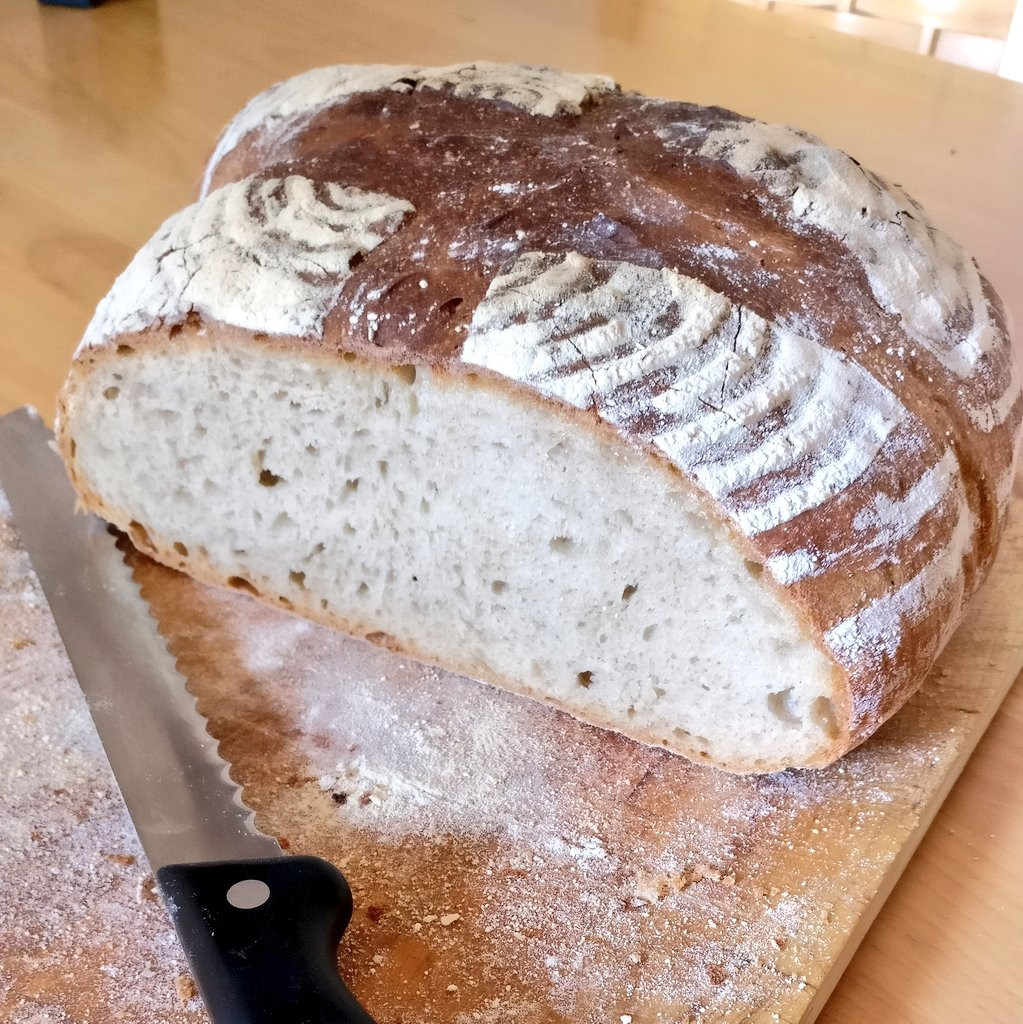
\includegraphics[height=\textheight]{hirabread/EV0I-6cUcAkaNUL.jpg}}
	    \end{figure}
	    
		\ingredients[14]{
		    \multicolumn{2}{c}{\textbf{Rye preferment}} \\
		    \SI{120}{\gram} & Rye flour 1150 \\
		    \SI{100}{\gram} & Water \\
		    \SI{8}{\gram} & Starter \\
		    & \\
		    \multicolumn{2}{c}{\textbf{Wheat preferment}} \\
		    \SI{75}{\gram} & Wheat flour 550 \\
            \SI{75}{\gram} & Water \\
            \SI{0.1}{\gram} & Fresh baker's yeast \\
            & \\
            \multicolumn{2}{c}{\textbf{Main dough}} \\
            \SI{375}{\gram} & Wheat flour 1050 \\
            \SI{125}{\gram} & Wheat flour 550 \\
            \SI{13}{\gram} & Salt \\
            \SI{6}{\gram} & Fresh baker's yeast \\
            \SI{300}{\gram} & Water 
		}
		
		\preparation {
		    \step Mix the rye dough and let ferment for \SI{18}{\hour} at a falling temperature, from \SIrange{30}{20}{\celsius}.
		    \step Mix the wheat dough and let ferment for \SI{18}{\hour} at \SI{20}{\celsius}.
		    \step Knead the dough and rest for \SI{45}{\minute} at \SI{24}{\celsius}.
		    \step Shape the dough, let rest for \SI{50}{\minute} at \SI{24}{\celsius}.
		    \step Bake the dough, with seam down, and scored with a cross, starting at \SI{280}{\celsius}, falling to \SI{200}{\celsius} for \SI{60}{\minute}.
		}
\end{recipe}
    \clearpage
	\begin{recipe}
[ %
        preparationtime = {\SIrange{3}{5}{\hour}},
        portion = {\portion{4--5}},
        source = {HeNine}
    ]{Goulash}

        \begin{figure}[p]
	        \centering
	        \makebox[\textwidth][c]{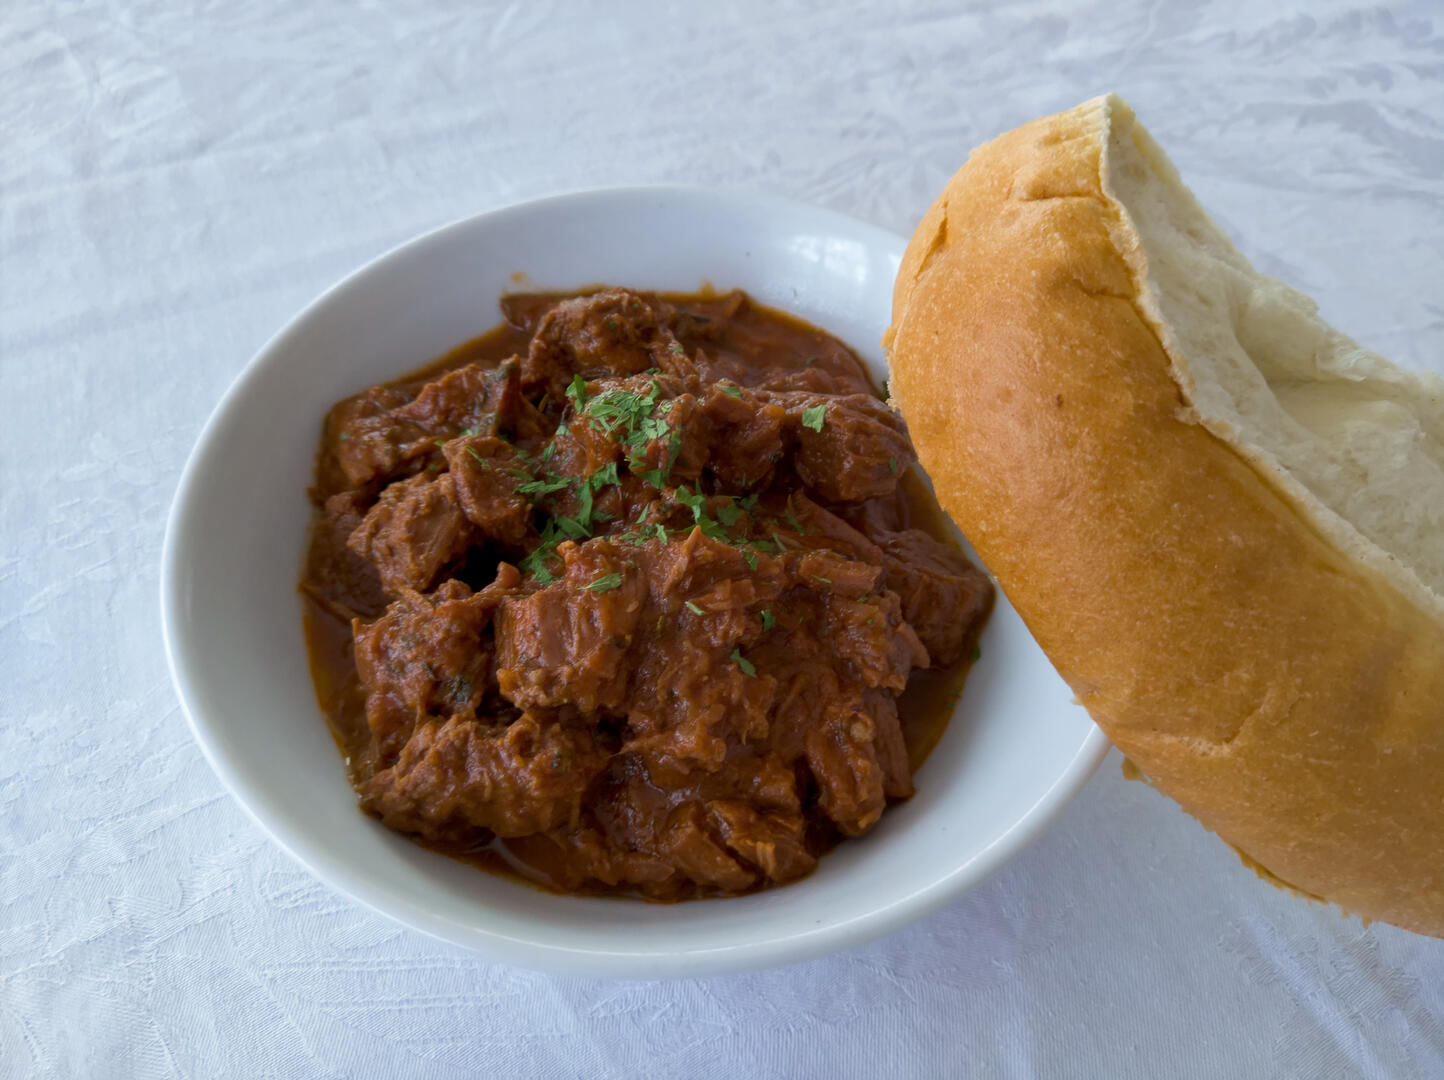
\includegraphics[height=\textheight]{goulash/IMG_20200202_120631.jpg}}
	    \end{figure}

	    \introduction{%
	        \textbf{\large BEEF}

	        Use a cheaper cut of meat, like thigh, flank or shoulder. You'll be stewing it to soften and adding lots of spices to maximize the taste.

            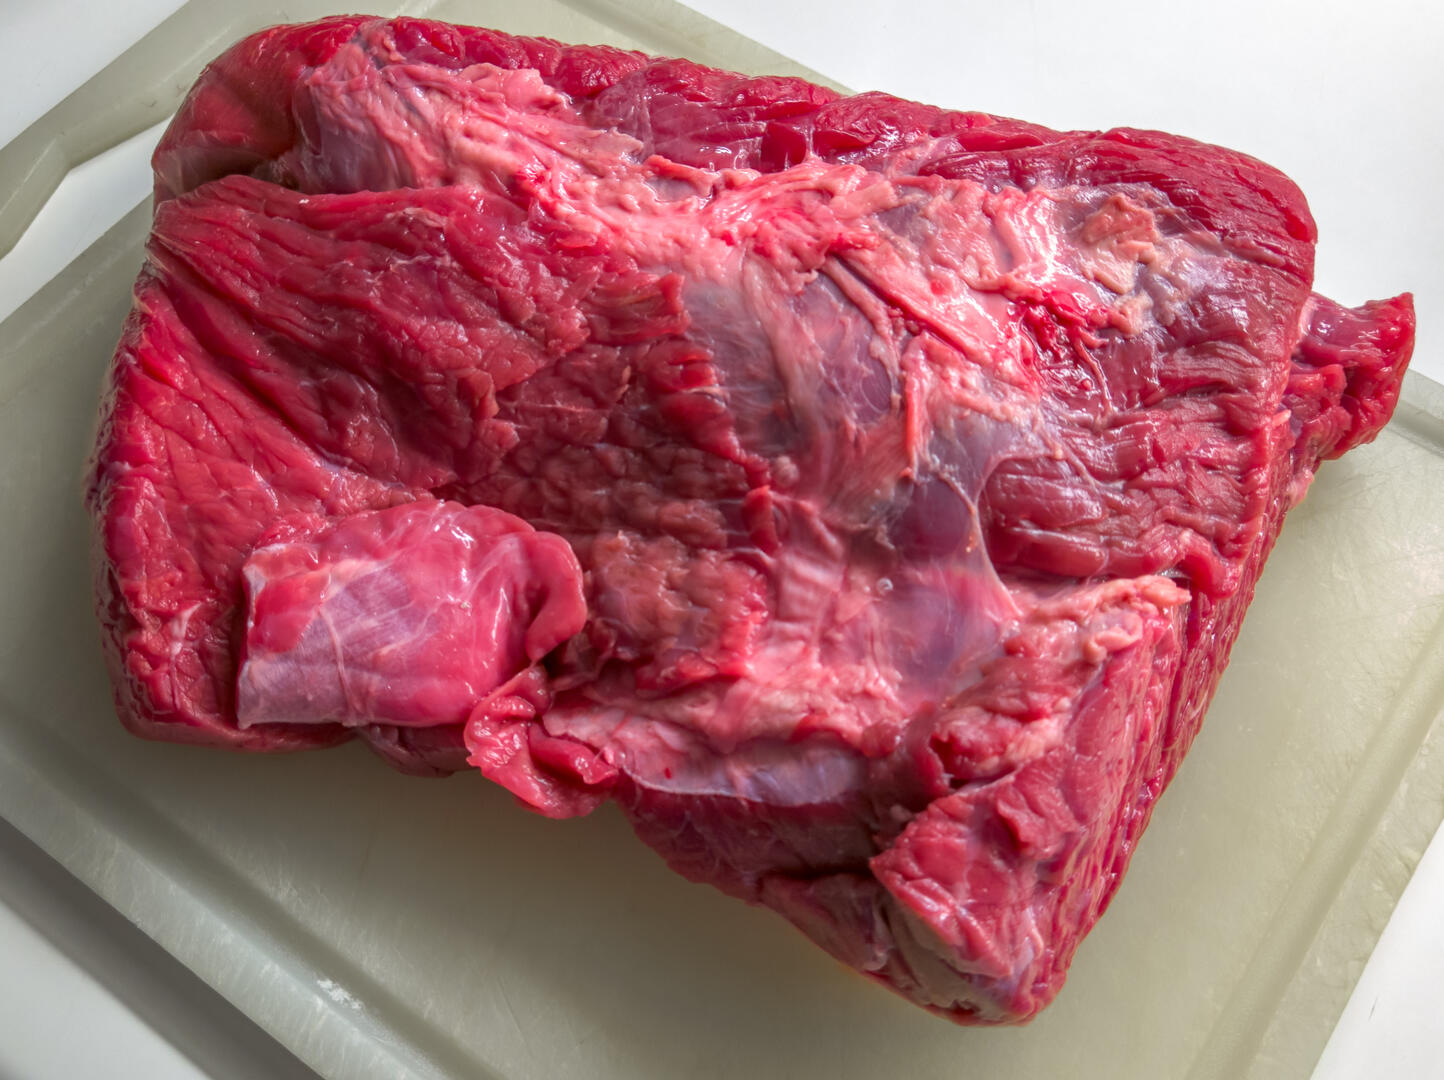
\includegraphics[width=\textwidth]{goulash/IMG_20200202_084818.jpg}

            \textbf{\large Onion}

            This is a pretty flexible recipe. You can use anywhere between 0.3 and 1.5 kg (per 1 kg of meat). I like a meatier version and onions make me farty.

            You can also use red or white or yellow onions OR A MIX! Fuck this boi up with onions!

            \newpage
            \textbf{\large Spice mix}

            The amounts here are eyeballed and I tend to go easy on cumin, but this mix works for me.

            Because we stew the meat for a long time I try to leave the herbs and spices in larger chunks: whole juniper berries, whole bay leaf, whole peppercorns, whole slightly crushed garlic cloves; I haven’t tried whole cumin and caraway, but that should also work.

            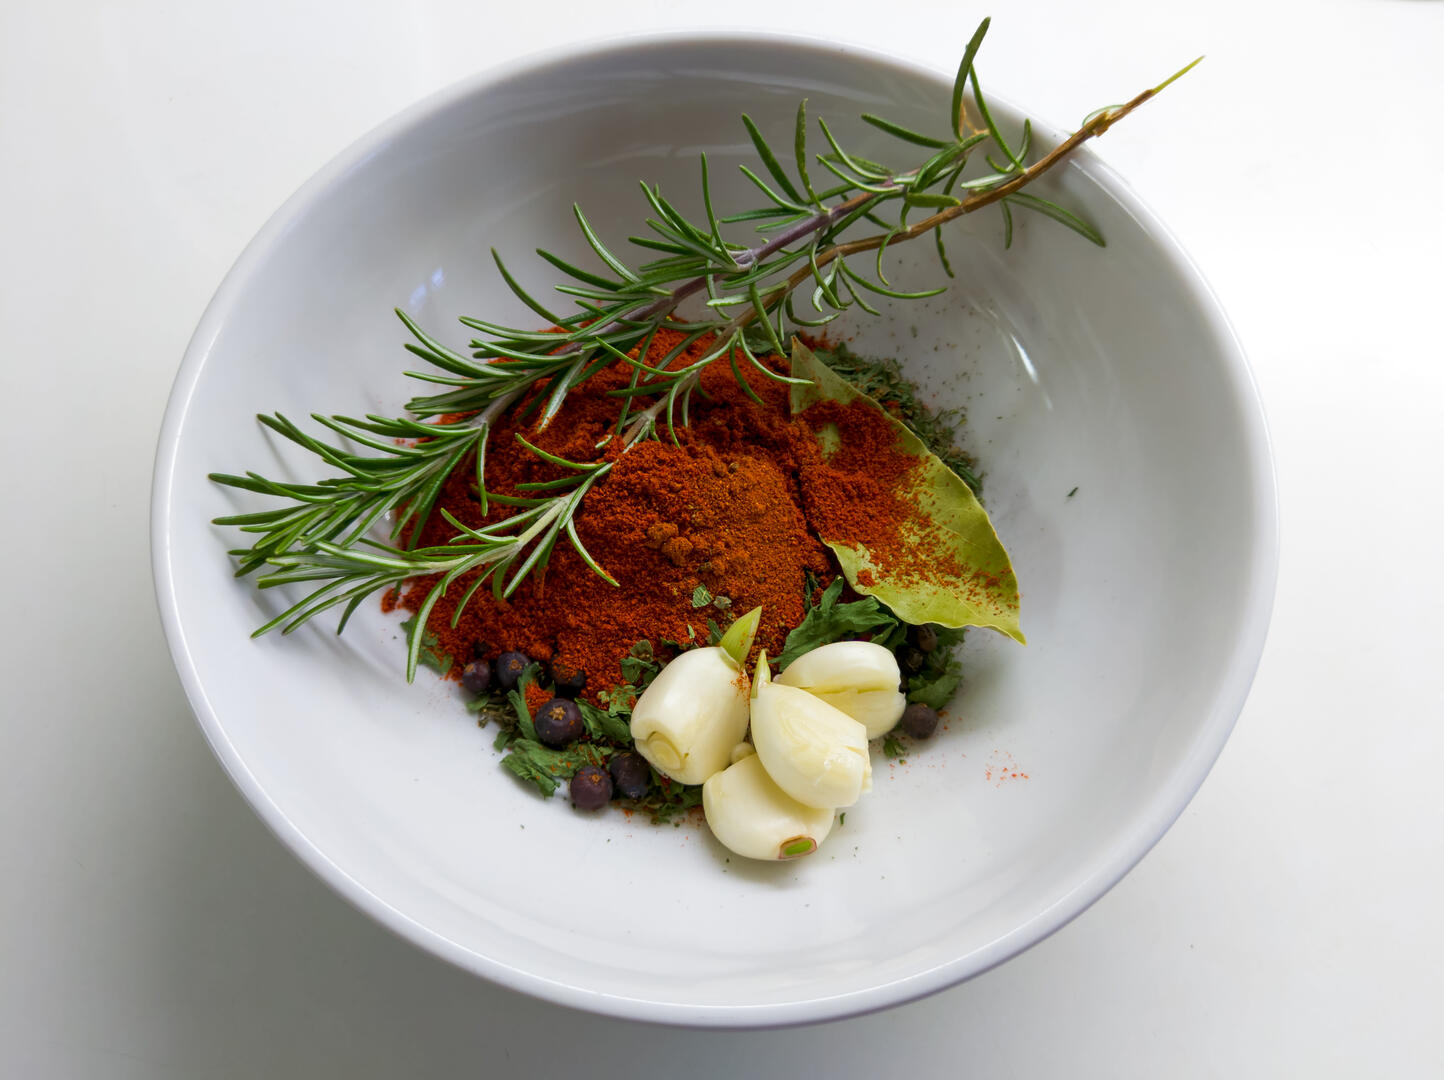
\includegraphics[width=0.5\textwidth]{goulash/IMG_20200202_095145.jpg}%
            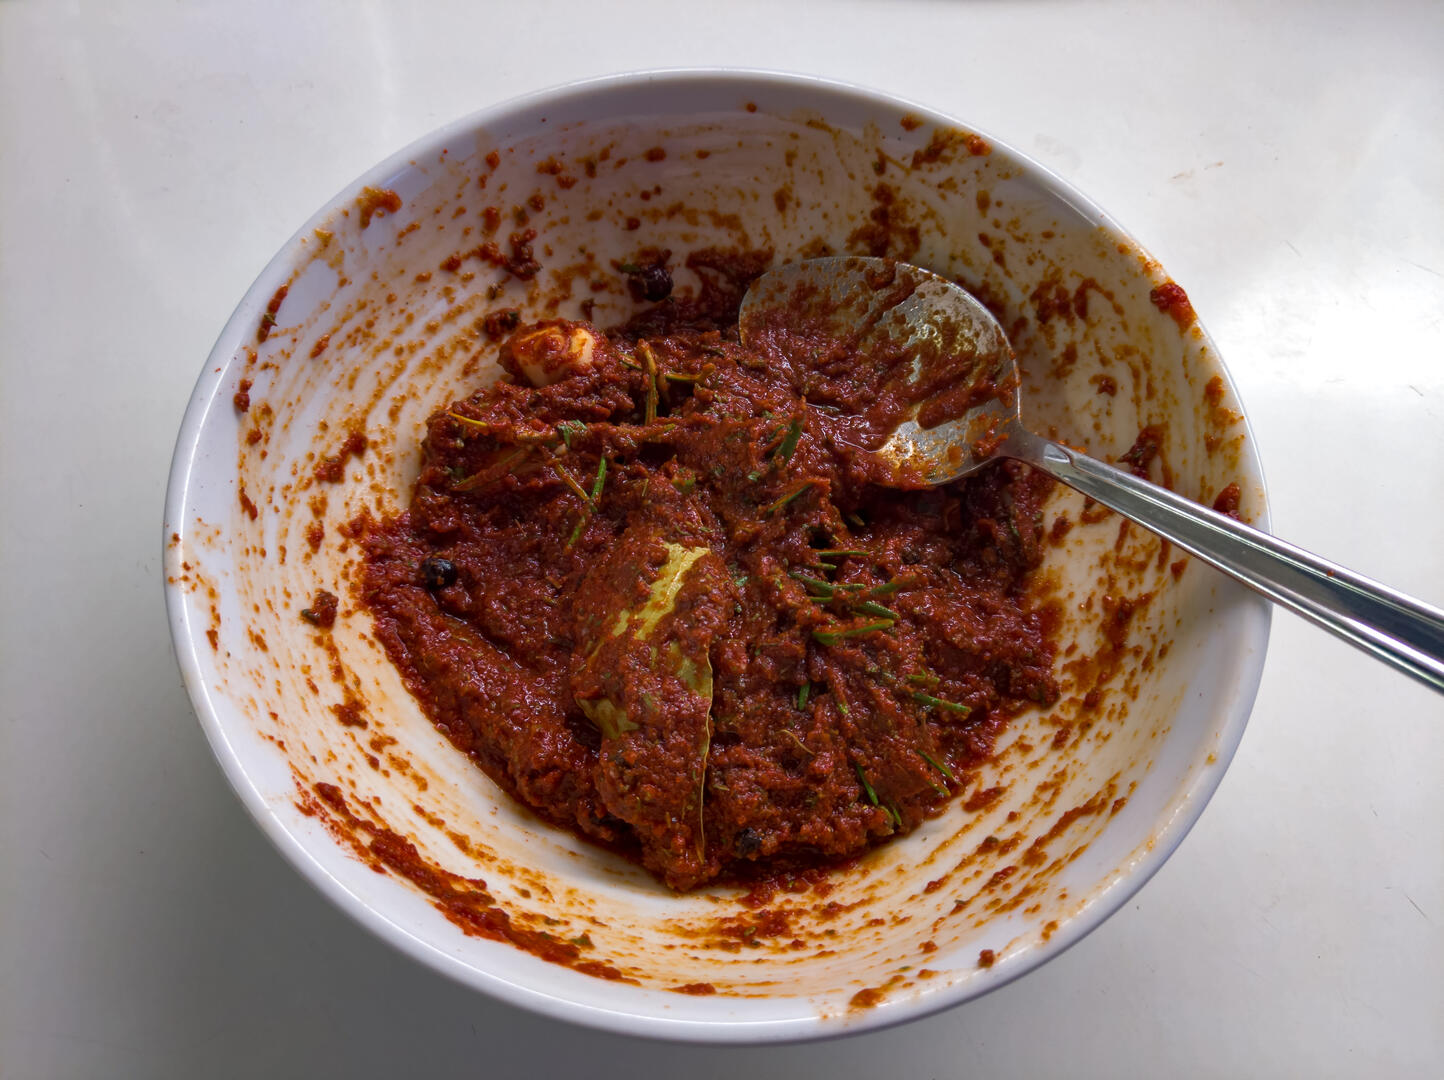
\includegraphics[width=0.5\textwidth]{goulash/IMG_20200202_095816.jpg}

            I pre-mix the spices with the tomato pur\'ee and the salt before adding them to the pot: mostly because I like how it looks and also to have something to do while the meat is browning.
	    }

	    \ingredients[16]{
            \SI{1}{\kilo\gram} & BEEF \\
            \SI{0.3}{\kilo\gram} & Onion \\
            1\,tsp & Thyme \\
            1\,tsp & Dry celery leaves \\
            1\,tsp & Summer savory (is apparently what it’s called) \\
            1\,tsp & Marjoram \\
            0.5\,tsp & Cumin \\
            1.5\,tsp & Caraway \\
            1\,large & Bay leaf or several small bay leaves \\
            idk some & Whole peppercorns \\
            7--10 & Juniper berries \\
            1.5\,tbsp & Paprika \\
            1\,sprig & Rosemary \\
            2\,cloves & Garlic \\
            1\,mTc & Salt! \\
            2\,tbsp & Tomato pur\'ee
        }

    \preparation{

        \step Clean and cut the meat into walnut-sized qubes. You don’t have to remove all fat and connective tissue, but the more you leave the longer it will take to render and soften.

%        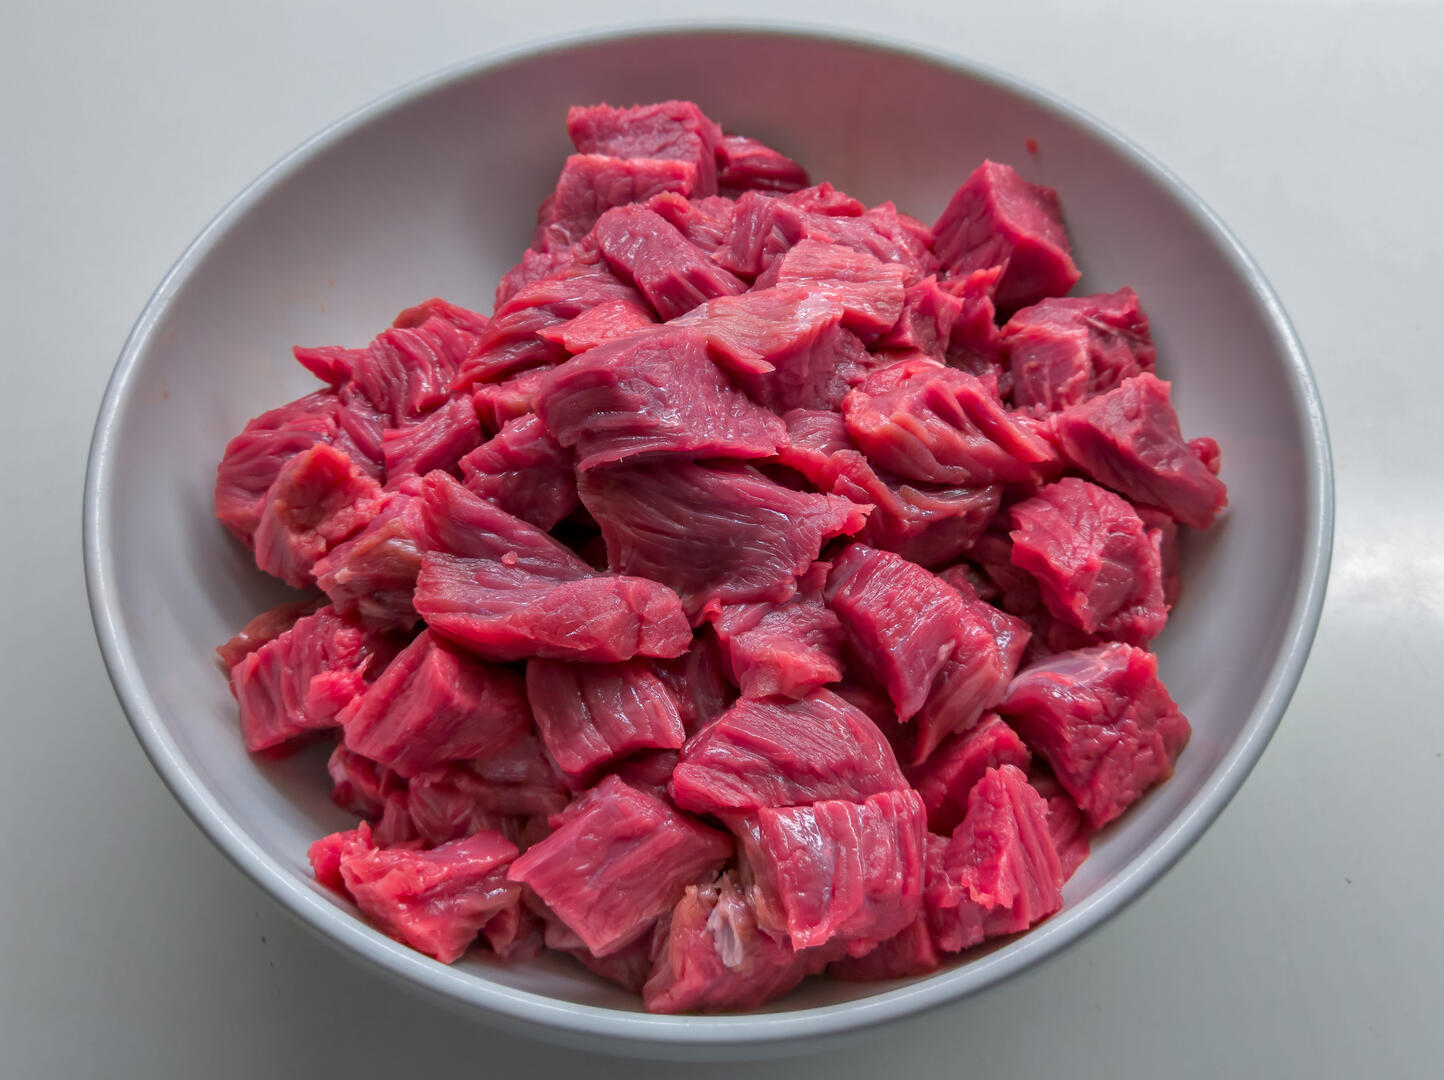
\includegraphics[width=0.53\textwidth]{goulash/IMG_20200202_091357.jpg}


        \step Slice the onions. The onions will ``melt'' while they cook, so you can chop them very roughly: small onions into quarters, larger onions lengthwise into 1 cm strips. Also, you’re cleaning and slicing like a kilogram of onions; you don’t wanna finely chop that many onions, do you?

%        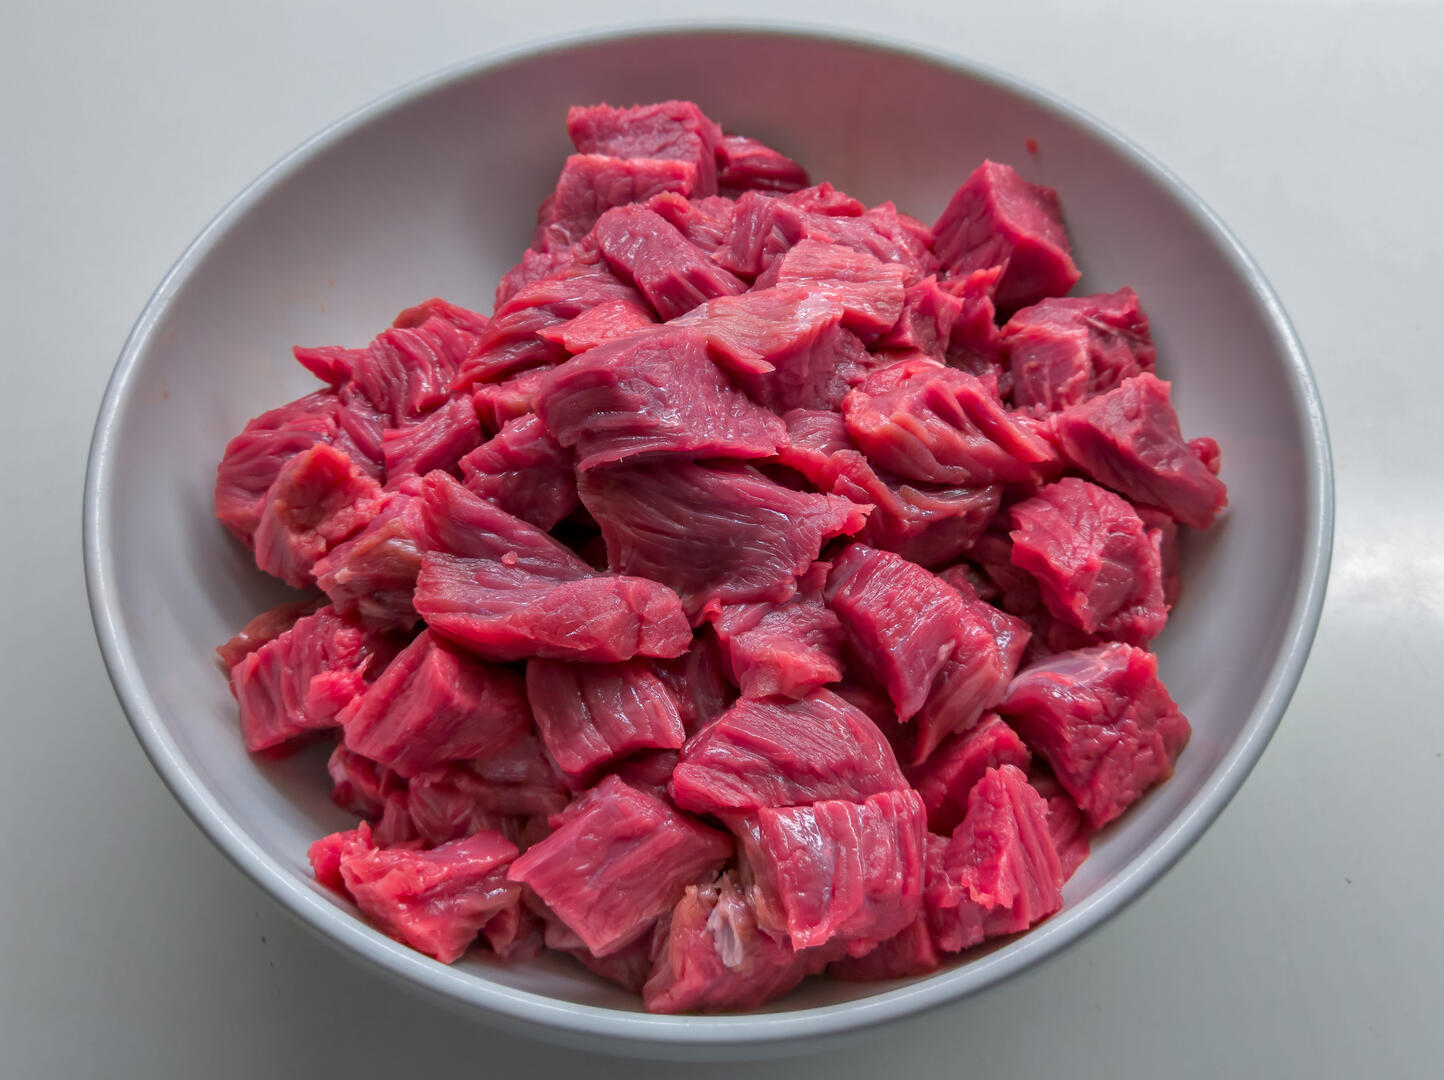
\includegraphics[width=0.5\textwidth]{goulash/IMG_20200202_091357.jpg}%
%        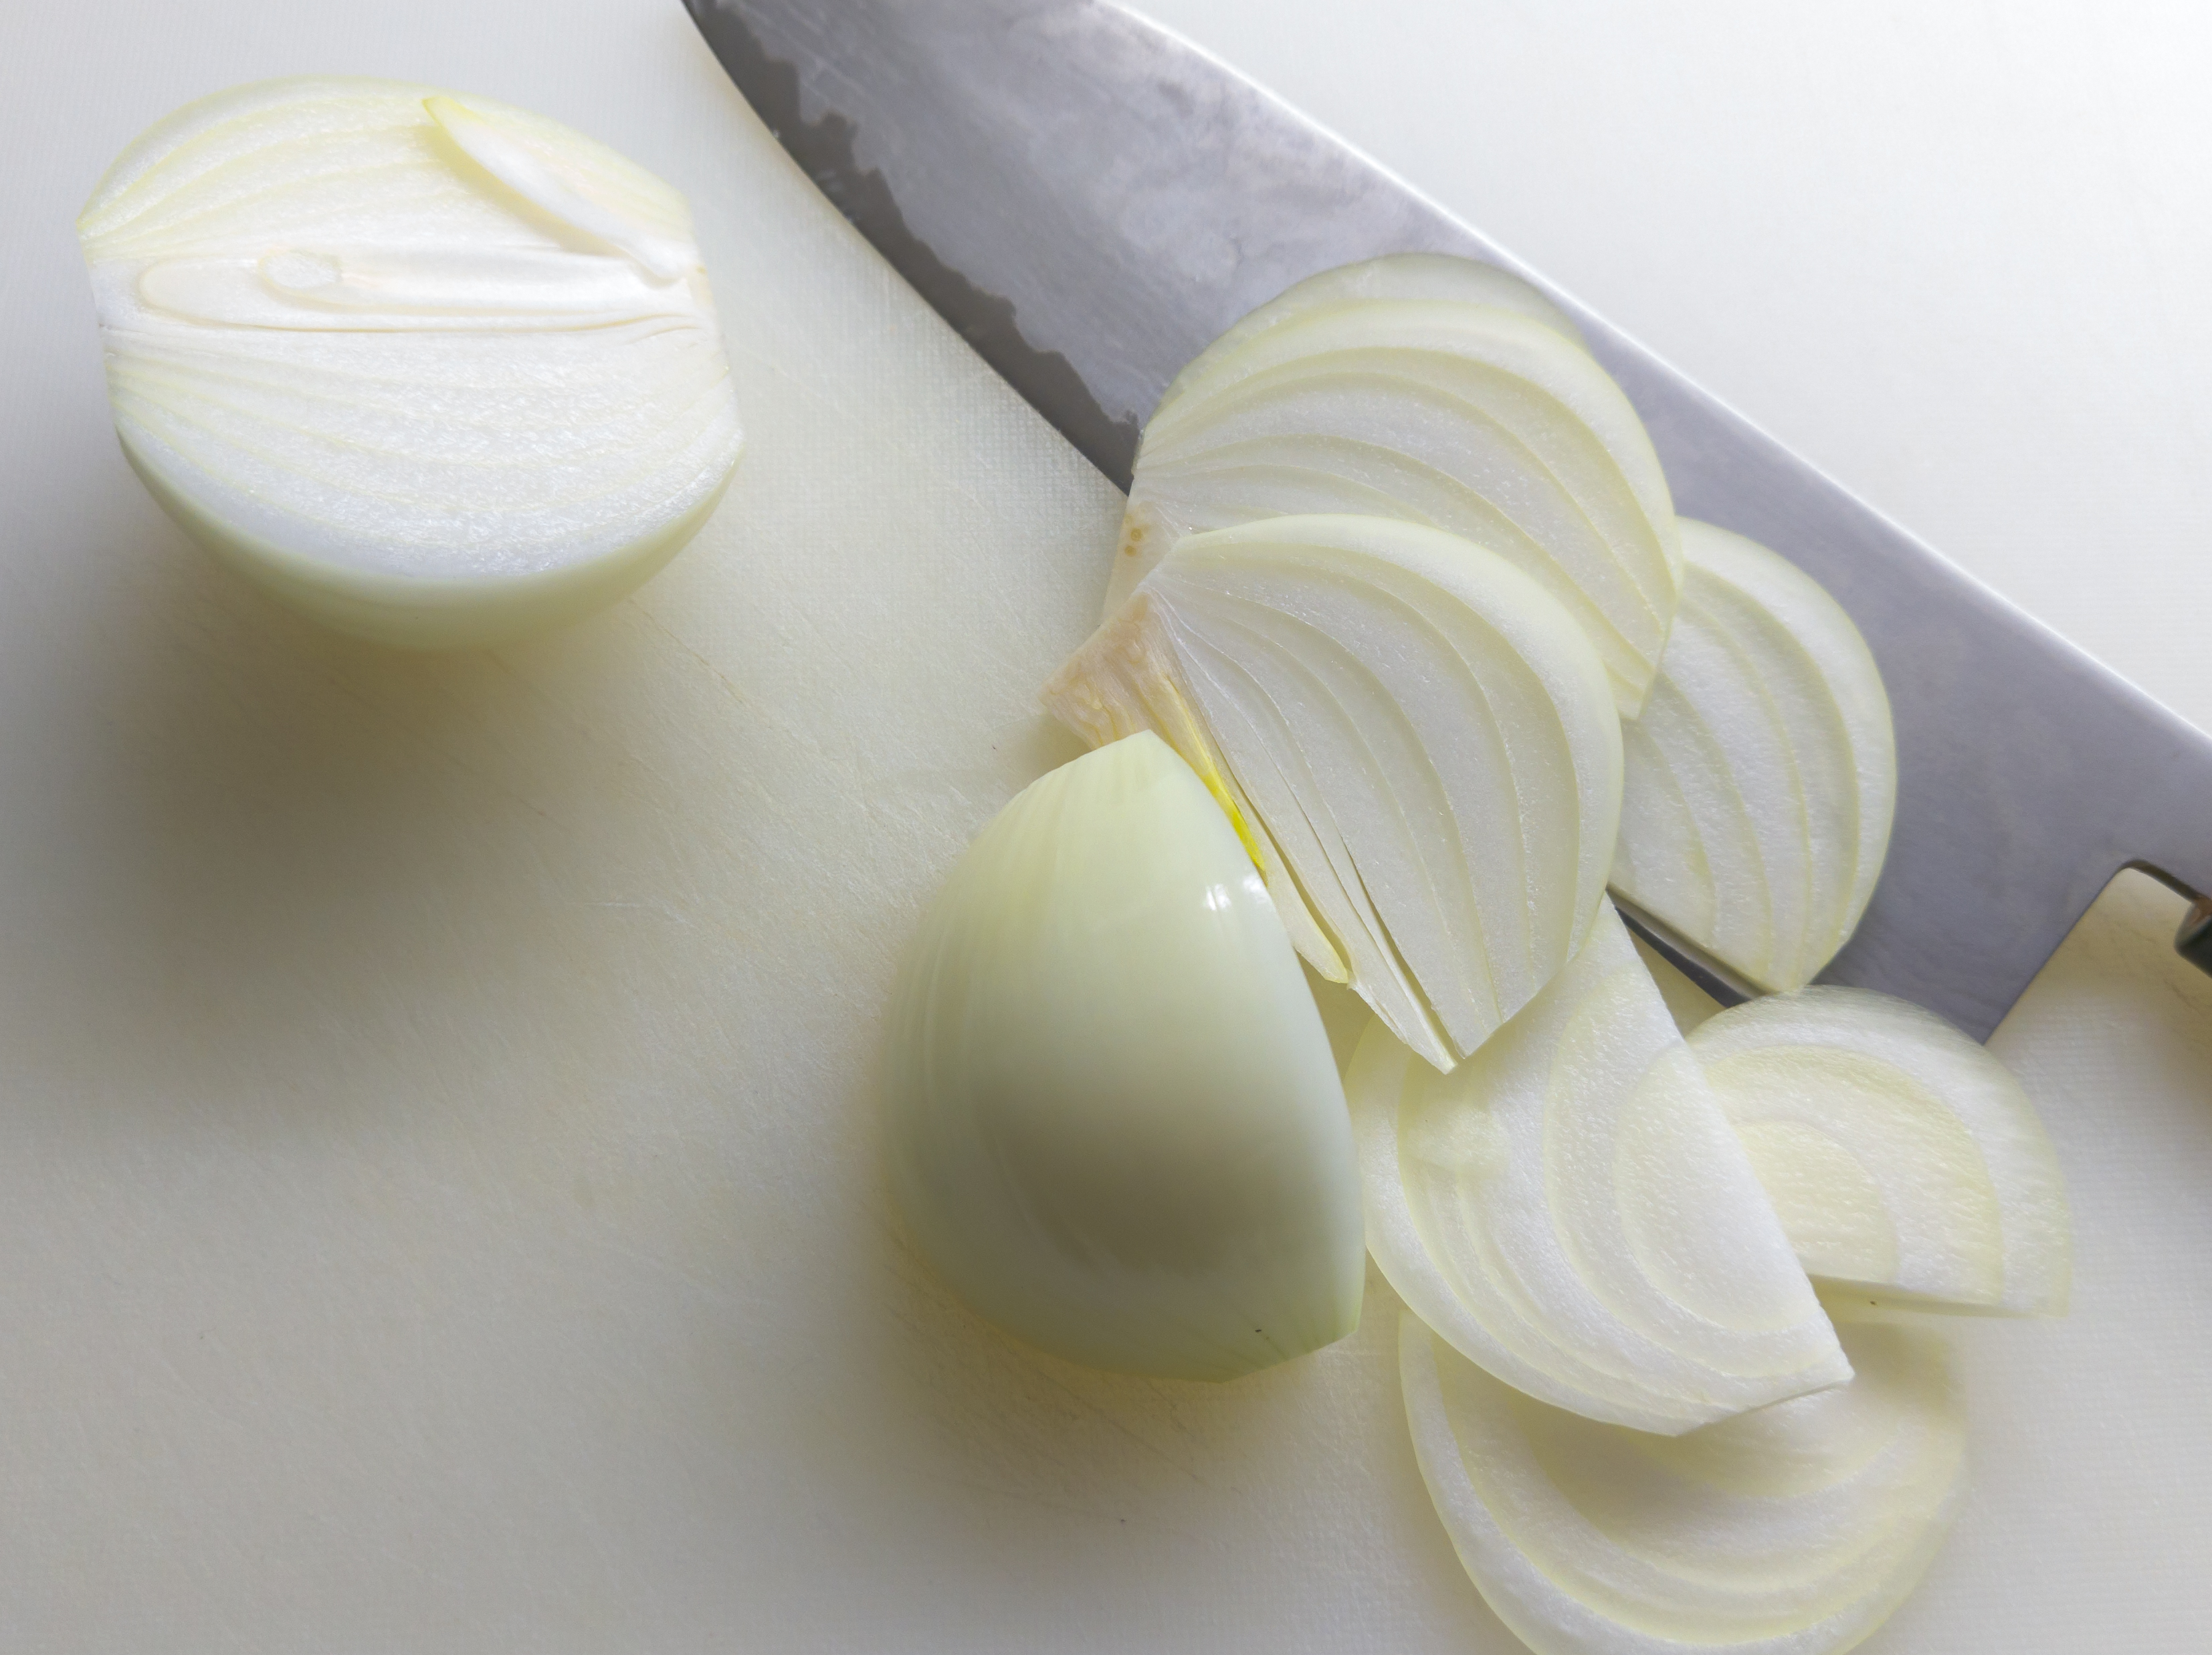
\includegraphics[width=0.5\textwidth]{goulash/IMG_20200202_091811.jpg}

%        \begin{wrapfigure}[11]{r}{0.51\textwidth}%
%            % \centering%
%            \hspace{-23pt}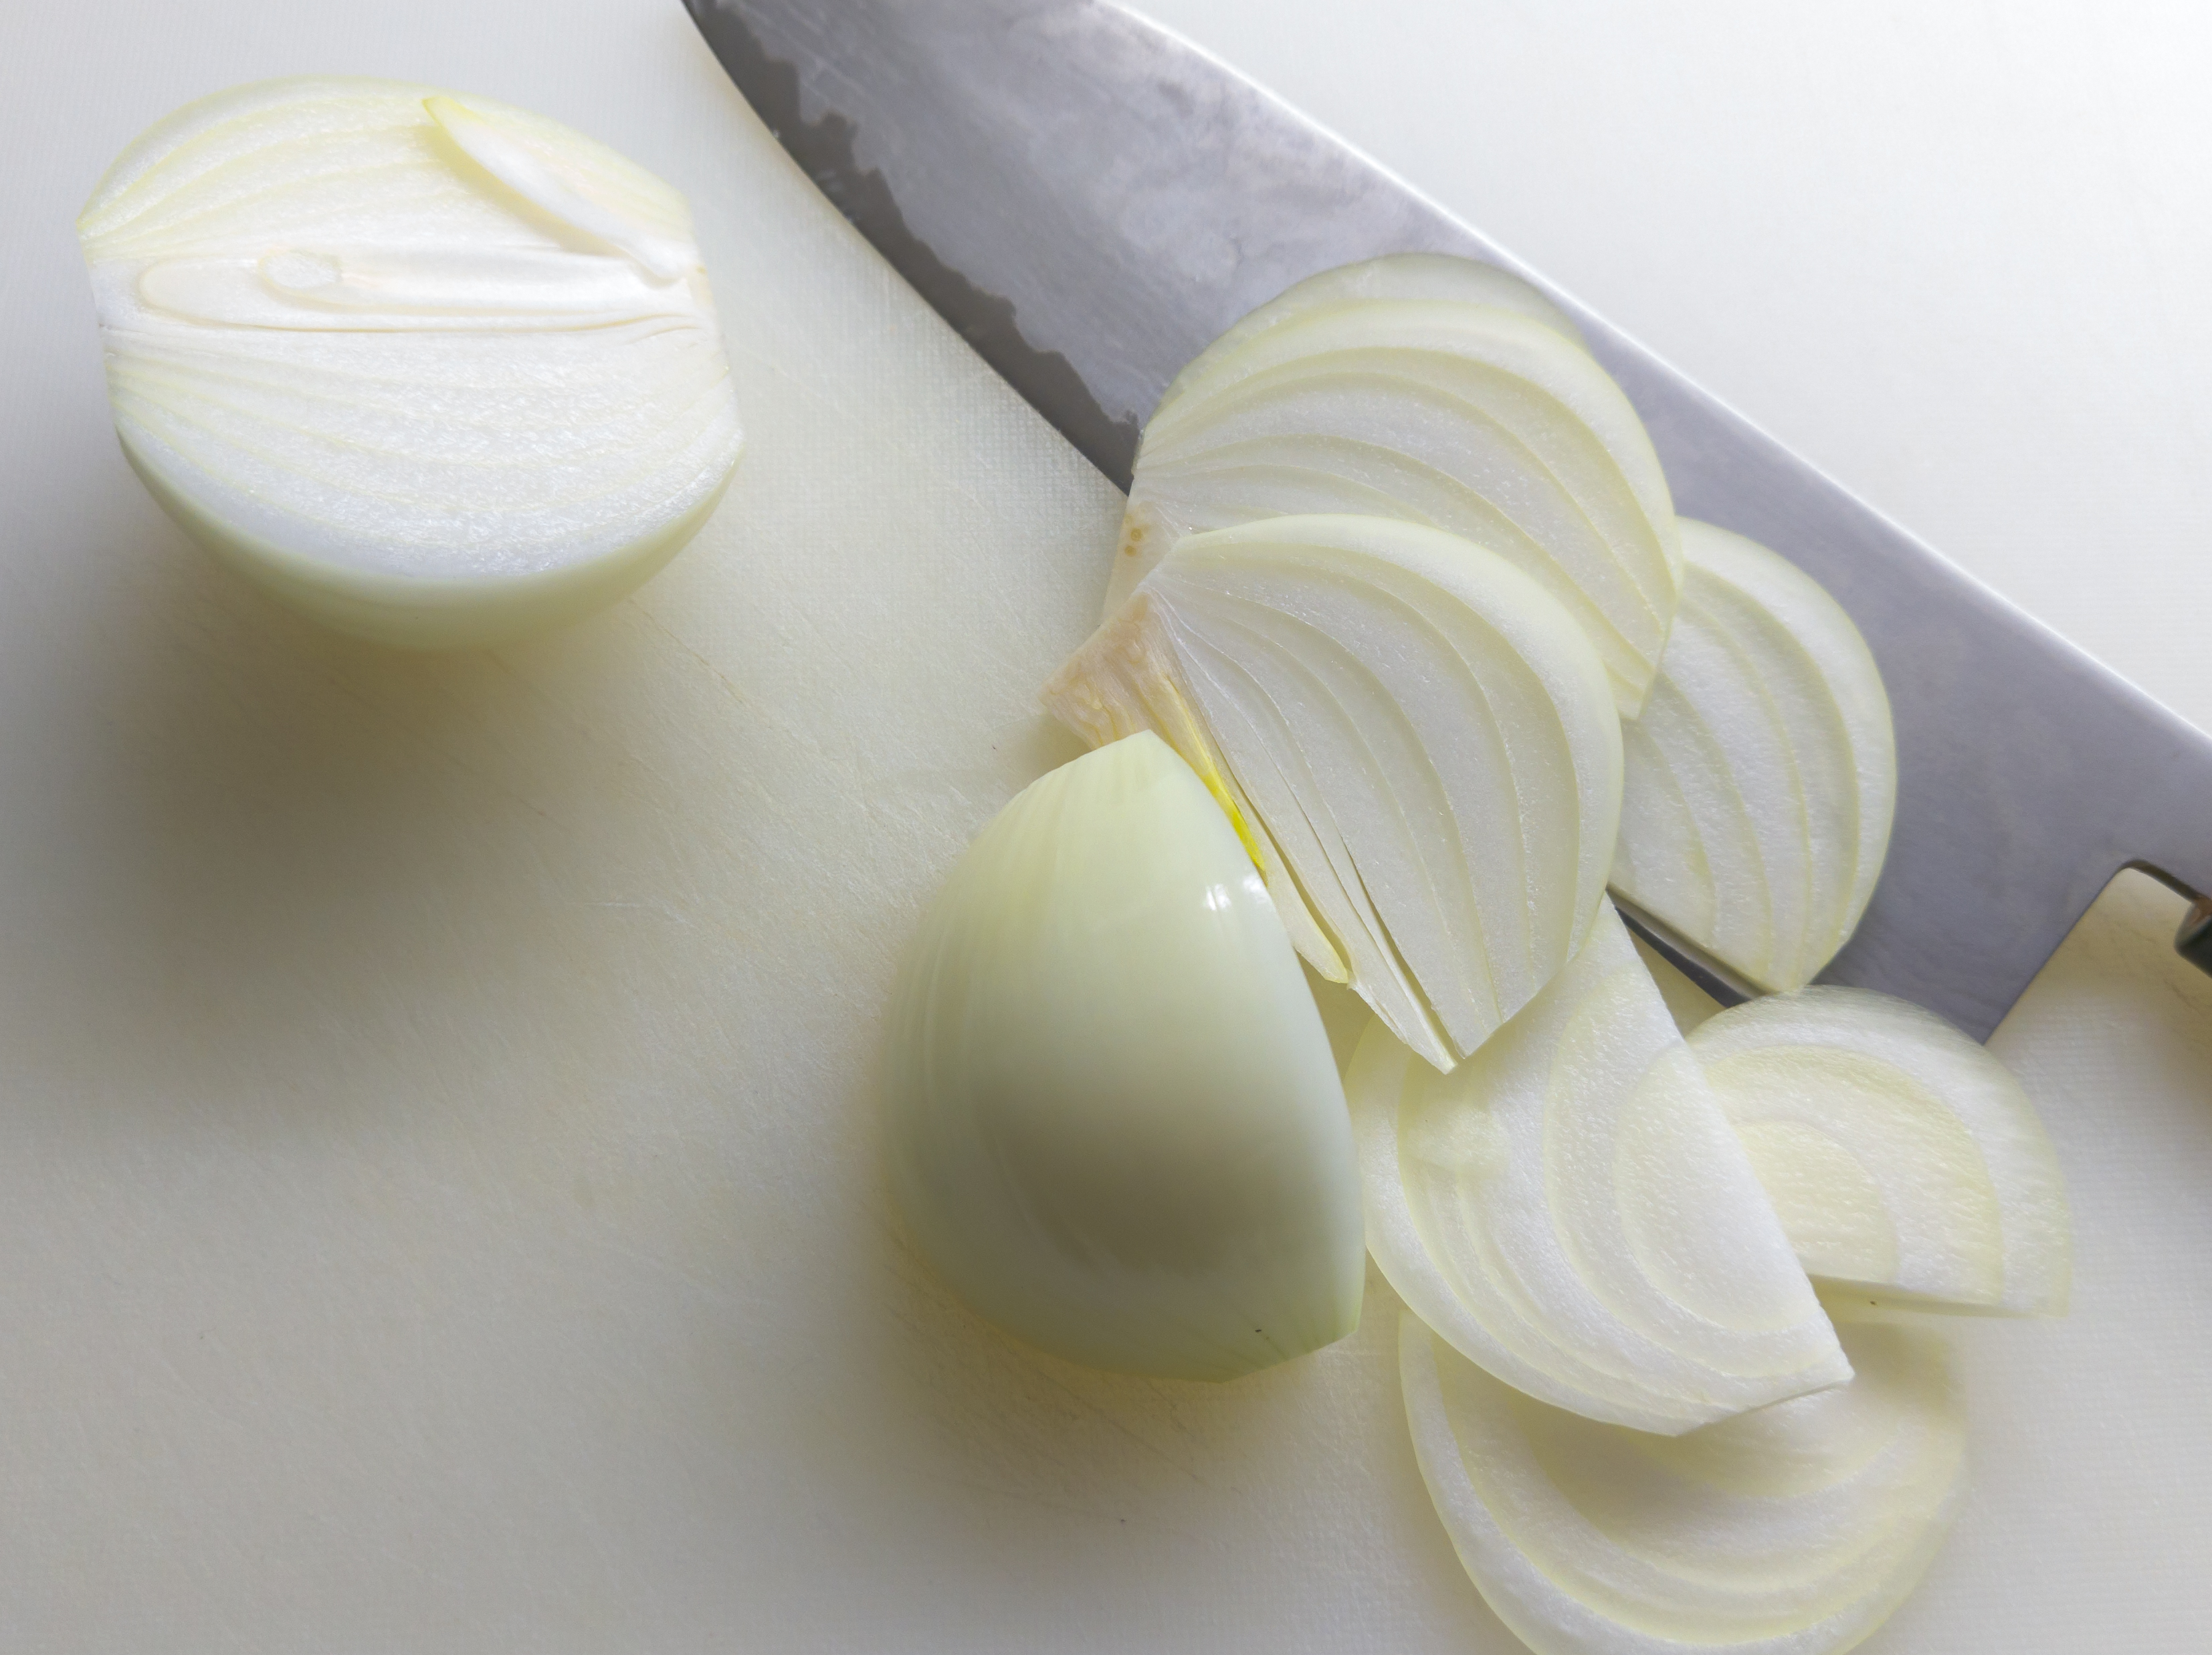
\includegraphics[width=0.5\textwidth]{goulash/IMG_20200202_091811.jpg}
%        \end{wrapfigure}

        \step Start saut\'eing the onions on high-mid heat on a bit of oil.

        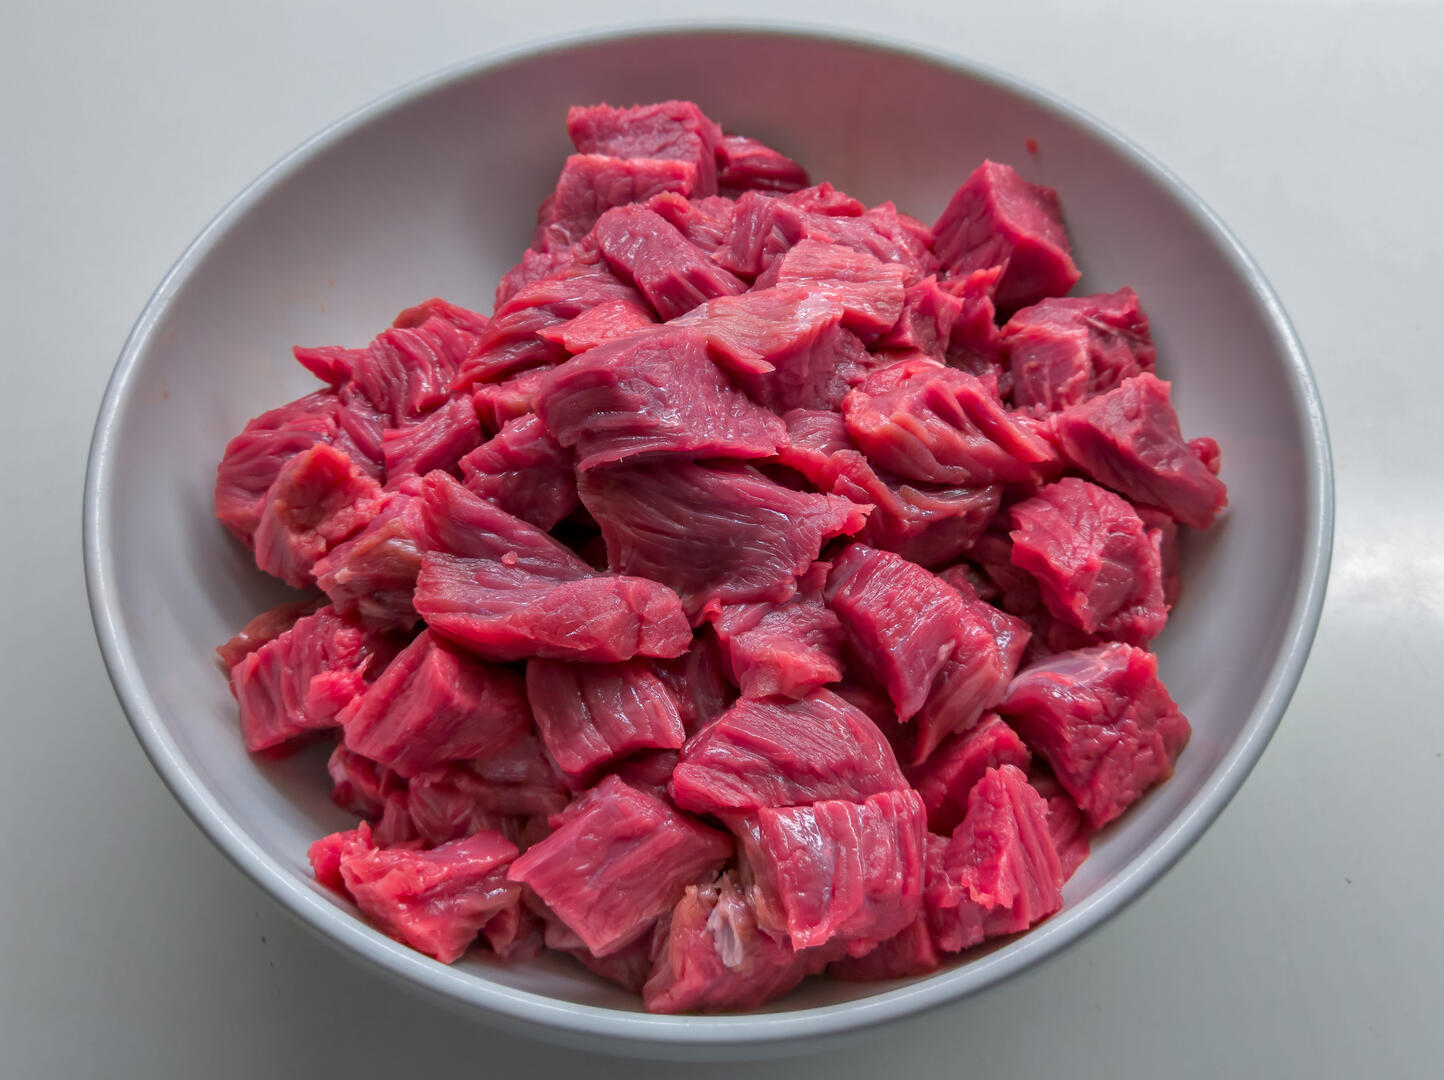
\includegraphics[width=0.5\textwidth]{goulash/IMG_20200202_091357.jpg}%
        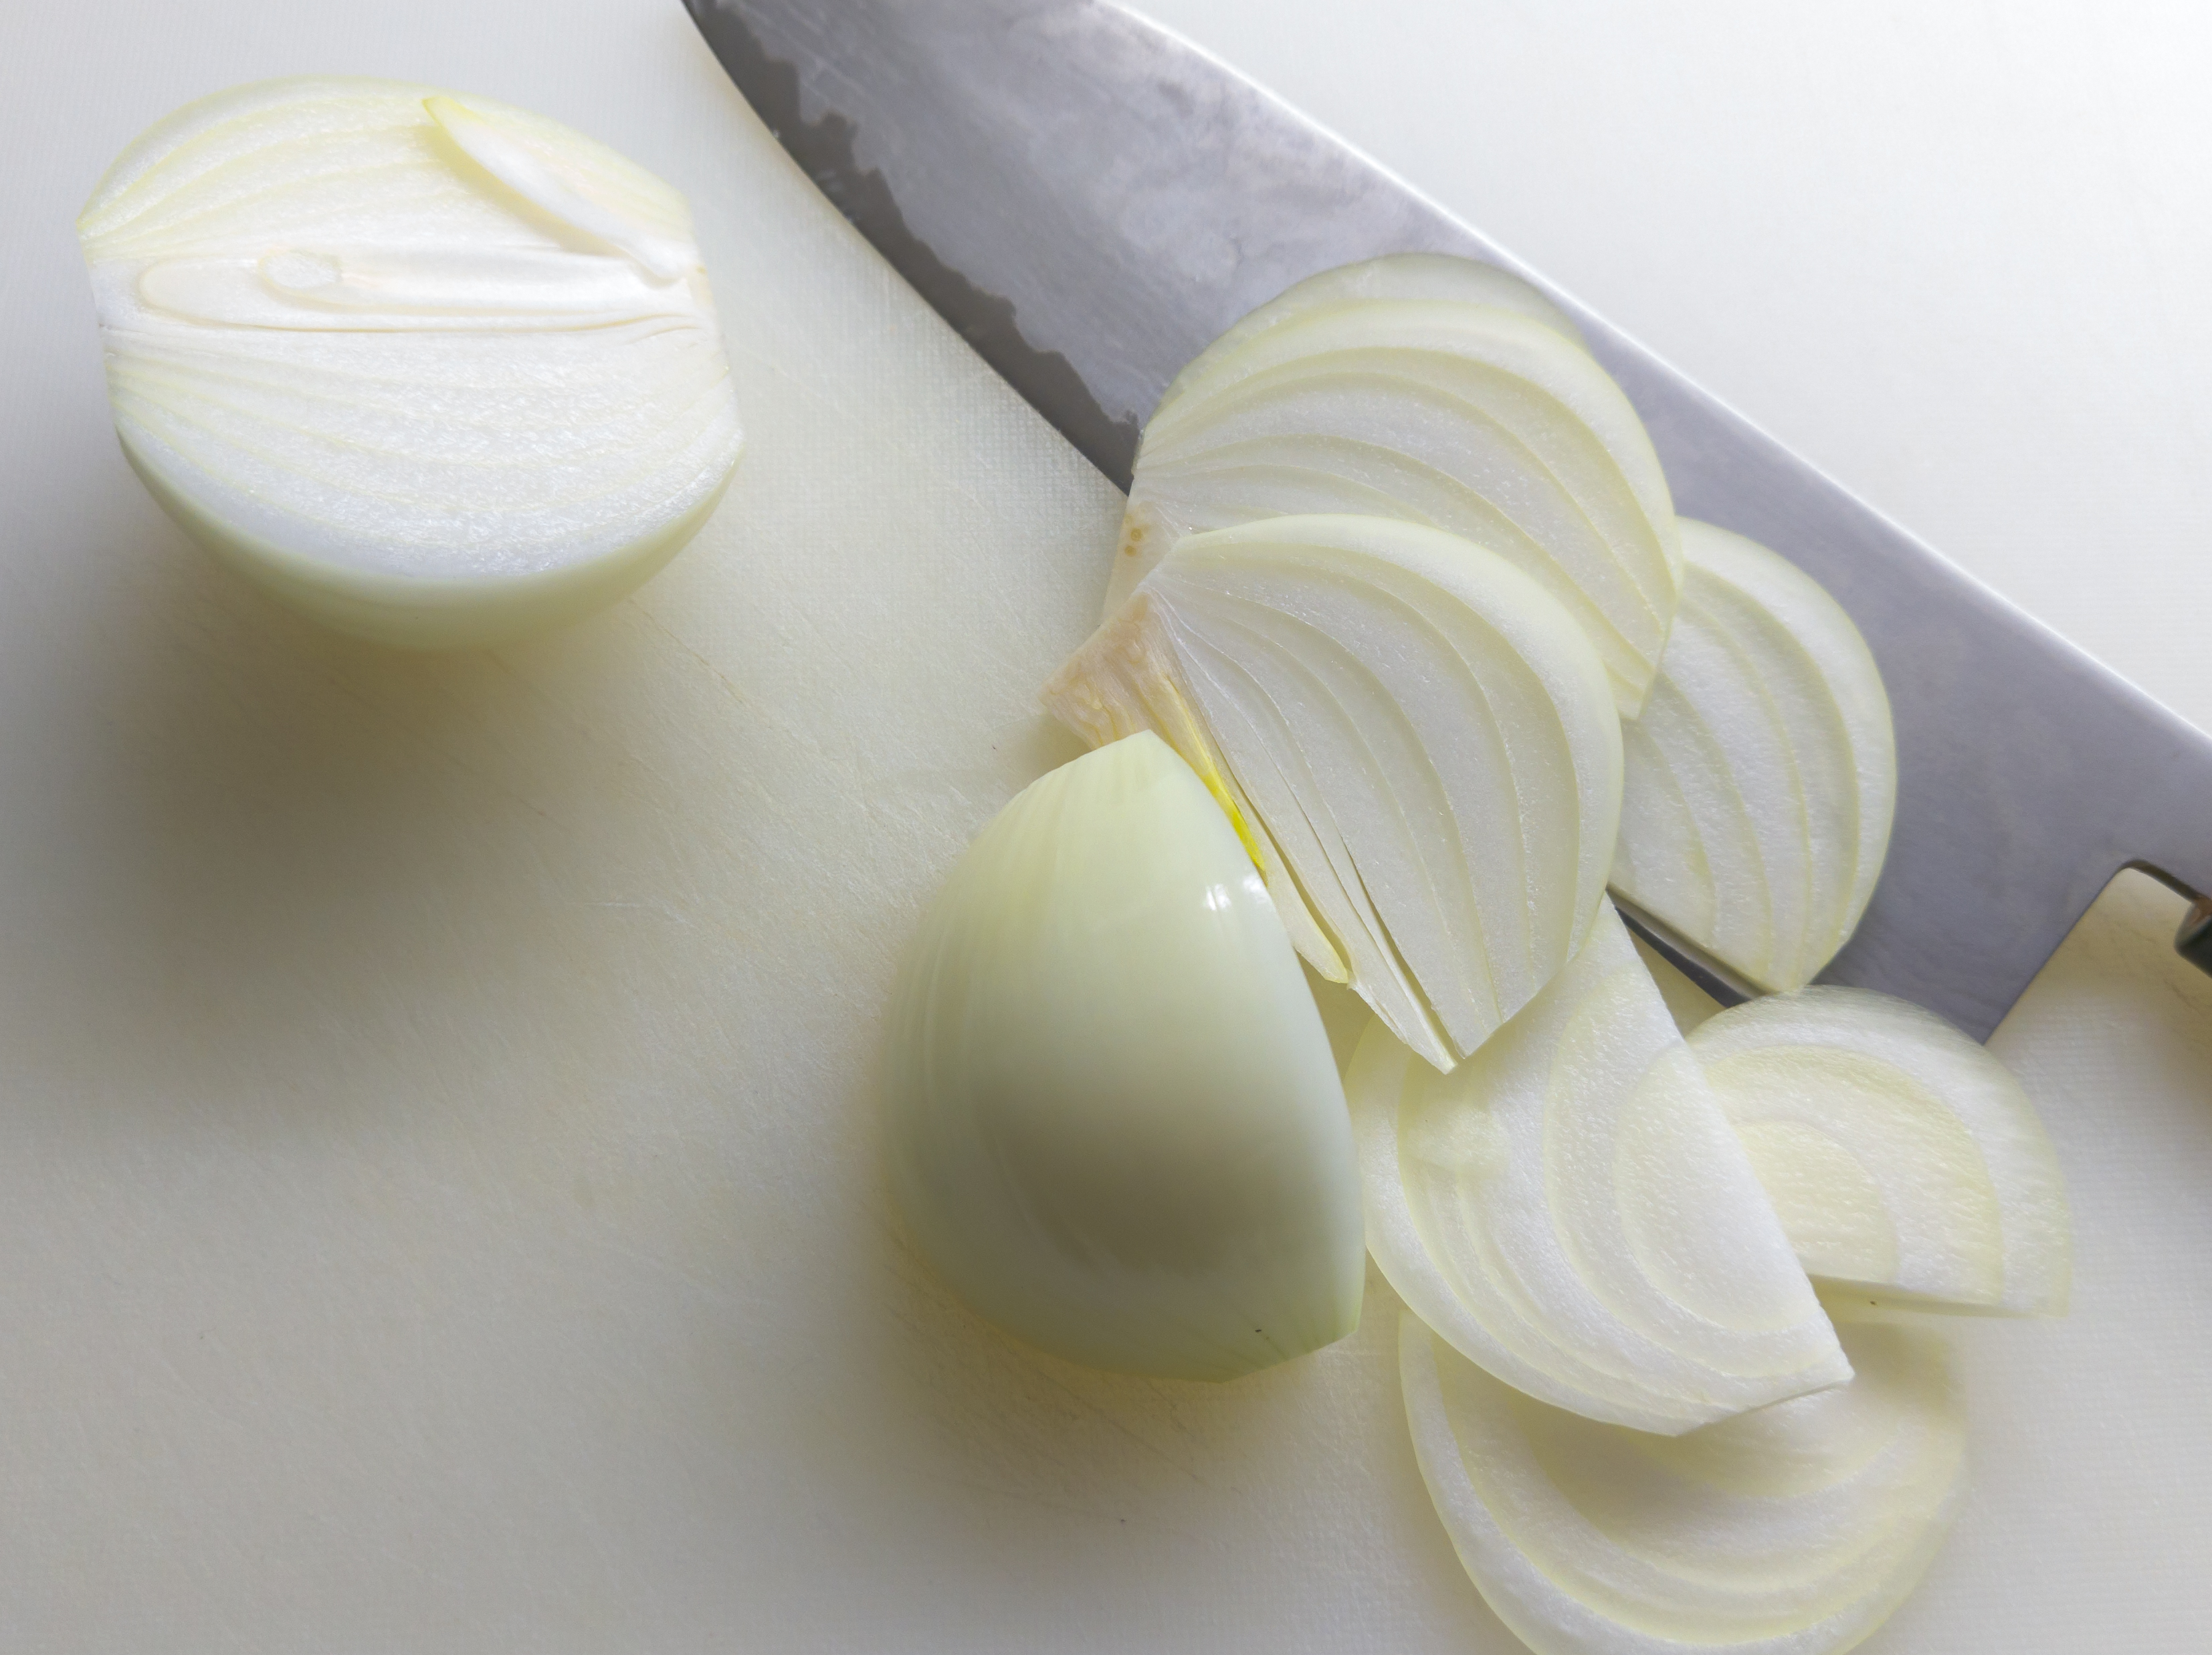
\includegraphics[width=0.5\textwidth]{goulash/IMG_20200202_091811.jpg}

%        \vspace{1em}

        \step When they start to brown add the meat. The meat will probably release a lot of liquid\footnote{ Normally, this effect, called ``crowding the pan,'' is bad as it can ruin the sear on a good steak, but in this case, we are going to stew the meat anyway, so it doesn’t change much.}. If that happens, raise the temperature and boil it off until it turns dark brown. This can take \textit{quite} a while. Otherwise, just brown the meat.

        \step Add wine and cook until it mostly boils off.

    	\vspace{1em}

        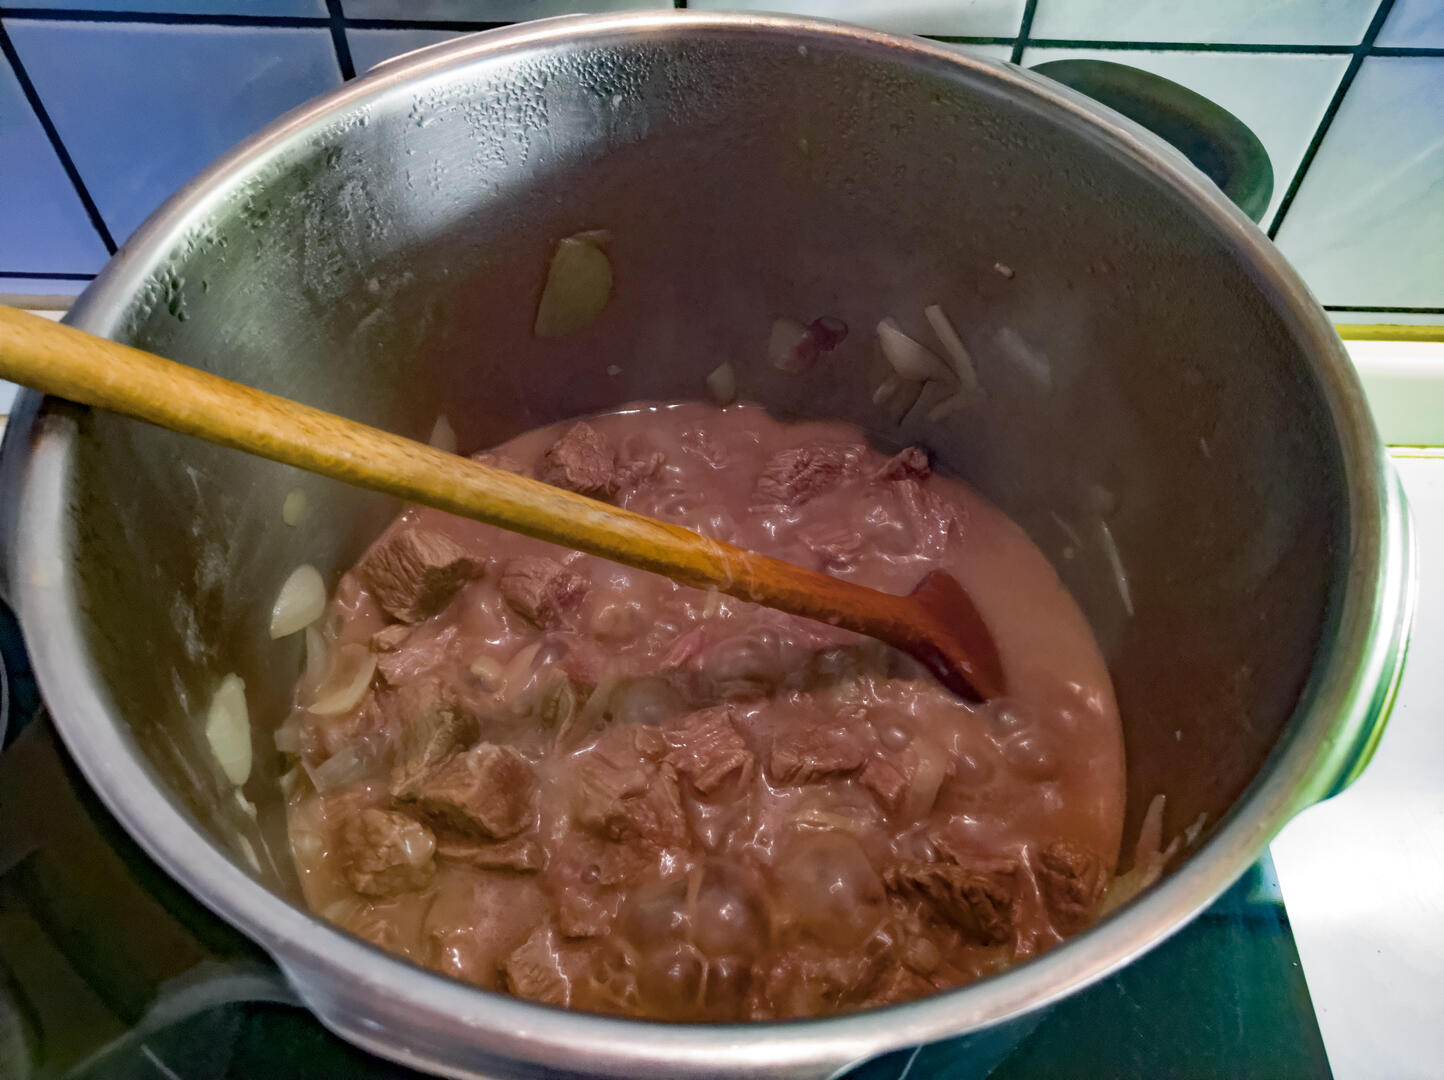
\includegraphics[width=0.5\textwidth]{goulash/IMG_20200202_095411.jpg}%
        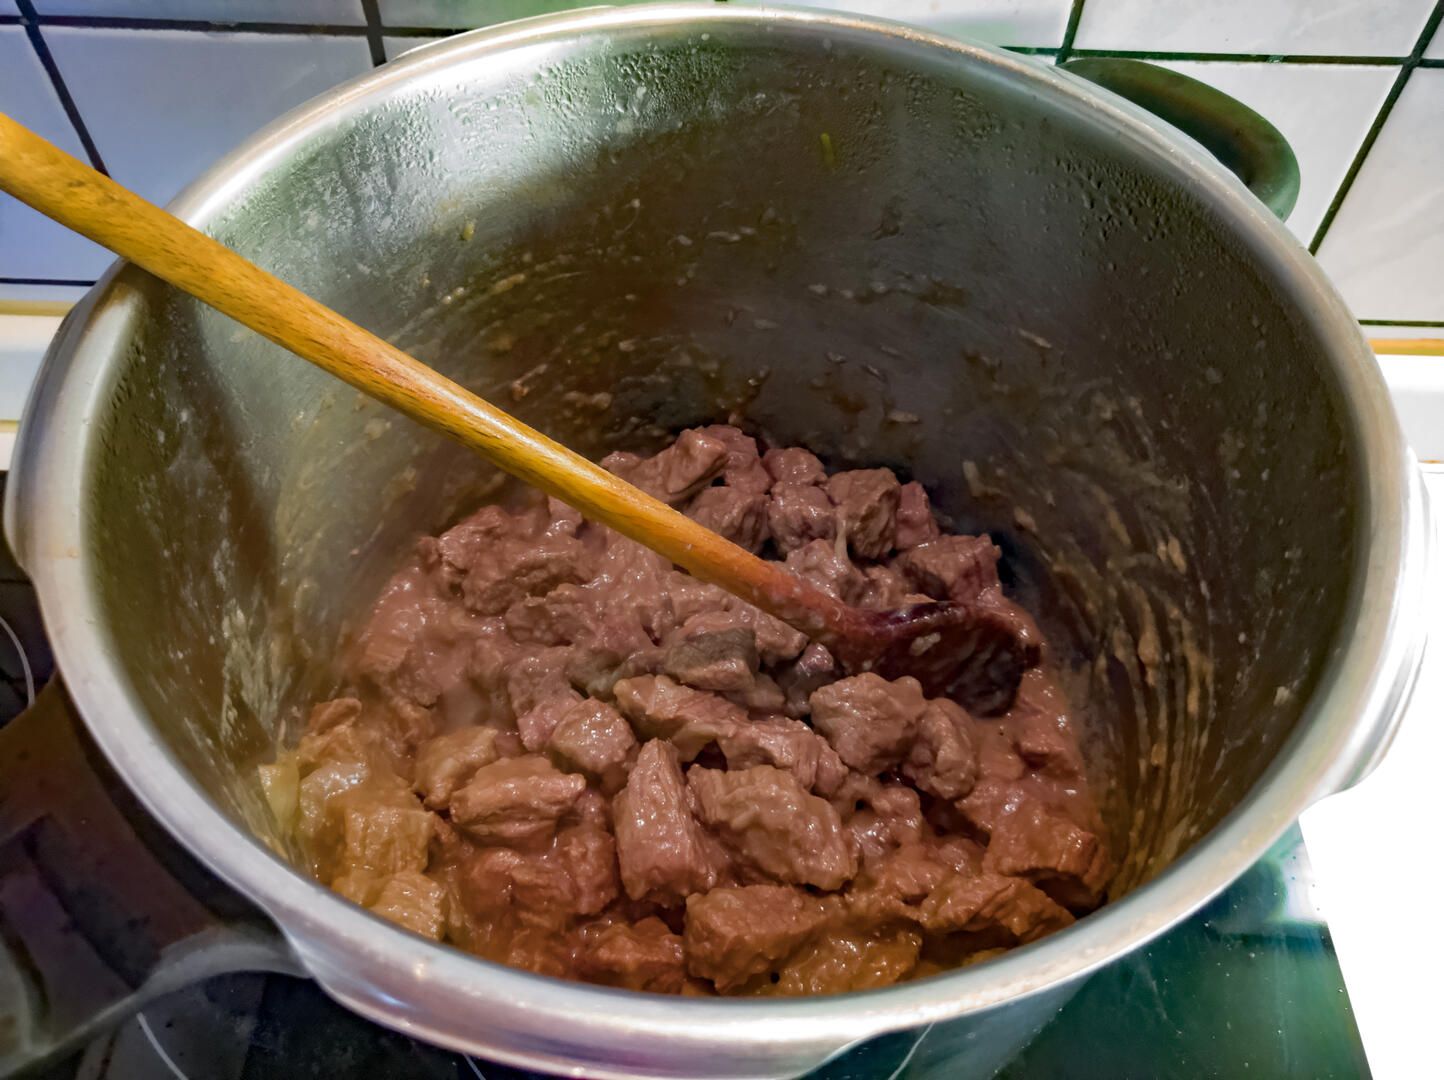
\includegraphics[width=0.5\textwidth]{goulash/IMG_20200202_101611.jpg}

        \step Add the spices with the salt and the tomato pur\'ee and add just enough water to cover everything.

        \step Keep simmering on low for at least 90 minutes; the longer the better. Keep adding water if too much boils off. If you’re using a pressure cooker you can shorten that time, but honestly, use the same time to get a better result.

        \step Serve. I like to have some nice bread with it, but gnocchi is also an option or some other pasta. Really, any starch works.
    }
\end{recipe}
    \clearpage
    \begin{recipe}
[ %
        preparationtime = {\SI{25}{\minute}},
        portion = {\portion[Human person, multiply as needed]{1}},
        source = {HeNine}
    ]{Pasta Carbonara}
       
      \begin{figure}[p]
	        \centering
	        \makebox[\textwidth][c]{\includegraphics[height=\textheight]{carbonara/IMG_20191220_124312-Edit(1).png}}
	    \end{figure}
       
    \introduction{%
        {\large\textbf{Meat}}
        
        Guanciale is traditional, but pancetta also works well. In a pinch, any pork product will work, especially good-old bacon or prosciutto.

        {\large\textbf{Salt}}
        
        The meat usually contains a lot of salt and so does the cheese, so you don’t need to add any, BUT if you use a less salty meat it doesn’t hurt to taste test.
    
        {\large\textbf{Cheese}}
        
        I use parmigiano, because it’s easier to get, but pecorino also works. You could probably get away with other cheeses as long as they melt and/or dissolve in the sauce. If you try cheddar please tell me about the results.
    }


    \ingredients[14]{
        1 & Small onion, the size of a medium onion\\
        \SIrange{80}{100}{\gram} & Meat \\
        50ish\, ml & White wine\\
        & Parmigiano to your heart’s content \\
        & Pepper just slightly over taste\\
        $1.54 \pm 1.05$\,tbs & Parsley\\
        & One (1) E G G. \\
        2--4\,tbsp & Olive oil \\
        \SI{90}{\gram} or so & Spaghetti (mom’s for preference, but store-bought is fine)
    }

    \preparation{
    \step Chop the onion and cut the meat into narrow strips. The thickness of the strips depends on the hardness of the meat: thin for pancetta, more cuboid for bacon or prosciutto.
    
    \step Saut\'e\footnote{The diacritic is crucial to the success of this dish.} the onions and the meat in a bit of oil\footnote{You can use olive oil if you can spare it, but a neutral oil like sunflower or canola works fine. Also note that if you use a fatty meat it will release its own fat so reduce the amount of oil accordingly.} until they just start to brown, then cover and keep on low-to-medium heat while stirring occasionally. A brown layer should be slowly building on the bottom of your pan.
    
    (You can use this time to prepare the sauce part and/or start cooking the pasta.)
    
    \step When the mixture is mostly brown add the wine to deglaze\footnote{While lacking in diacritics, this technique is just as important.} the pan. Leave on low heat until most of the wine has boiled away and you have a nice brown sauce with meat chunks.

    \step Keep warm, but not simmering until you are ready to combine.
    
    \vspace{1em}

    \step Stir together the cheese, E G G, olive oil, cracked or coarse-ground pepper (pepper, pepper) and parsley in a bowl and set aside. I recommend making the dish fairly peppery, but if you don’t like pepper feel free to adjust.
    
    If you are new to cooking I would recommend you prepare this before you start other things, but if you are comfortable in the kitchen you can do it while waiting for the meat to brown.

    \step Cook the paste to desired hardness according to manufacturer's instructions. I usually go for 1 minute less than specified.
    
    \step Do not rinse pasta in cold water.
    
    \vspace{1em}
    {\large\textbf{Combining}}
    
    \step Add the pasta to the meat and stir in the egg mixture. We are using the heat of the pasta and the meat sauce to cook the egg, so ensure that both are still hot.
    
    \step Cover and meditate on the nature and moral implications of protein coagulation and its relation to emulsification for \SIrange{2}{3}{\minute}, or however long it takes you to prepare the table or a salad, and get everyone to come to the table, if you are sharing this wonderful meal with other people, or just relax for a bit if you’re eating on your own.

    \textbf{Alternative:} you can also heat the whole mixture to completely cook the egg into a more scrambled egg texture, if you prefer that.

    \step Serve. You can garnish with a bit of parsley, if you feel like it or add a bit more cheese on the top, if you feel like it doesn’t already contain enough cheese.
    }
    
\end{recipe}
	\clearpage
	\begin{recipe}
[ %
        preparationtime = {\SI{1}{\hour}},
        portion = {\portion{1}},
        source = {mithodin},
        sourceref ={Tokyo Cult Recipes}
    ]{Japanese Potato and Beef Stew}

    \ingredients[8]{
        5--10 & Potatoes \\
        1 & Onion \\
        \SI{200}{\gram} & Beef \\
        \SI{350}{\milli\liter} & Dashi \\
        \SI{50}{\milli\liter} & Soy sauce \\
        \SI{50}{\milli\liter} & Sake  \\
        \SI{50}{\milli\liter} & Mirin \\
        2\,tbsp & Cane sugar
    }

    \preparation{
        \step Thinly slice the beef and give it some color.
        \step Add the potatoes (in large-ish chunks) and the onion (sliced), and give those a little bit of colour too.
        \step Add all the fluids and the sugar; boil on a medium-low heat for 10 minutes.
        \step Remove the lid and increase the heat to reduce the liquid down to about $2/3$.
    }

\end{recipe}
	\clearpage
	\begin{recipe}
[ %
        preparationtime = {\SI{1}{\hour}},
        portion = {\portion{Idk, how much do you like potatoes?}},
        source = {HeNine}
    ]{Pra\v{z}en krompir}
    
    \begin{figure}[p]
	        \centering
	        \makebox[\textwidth][c]{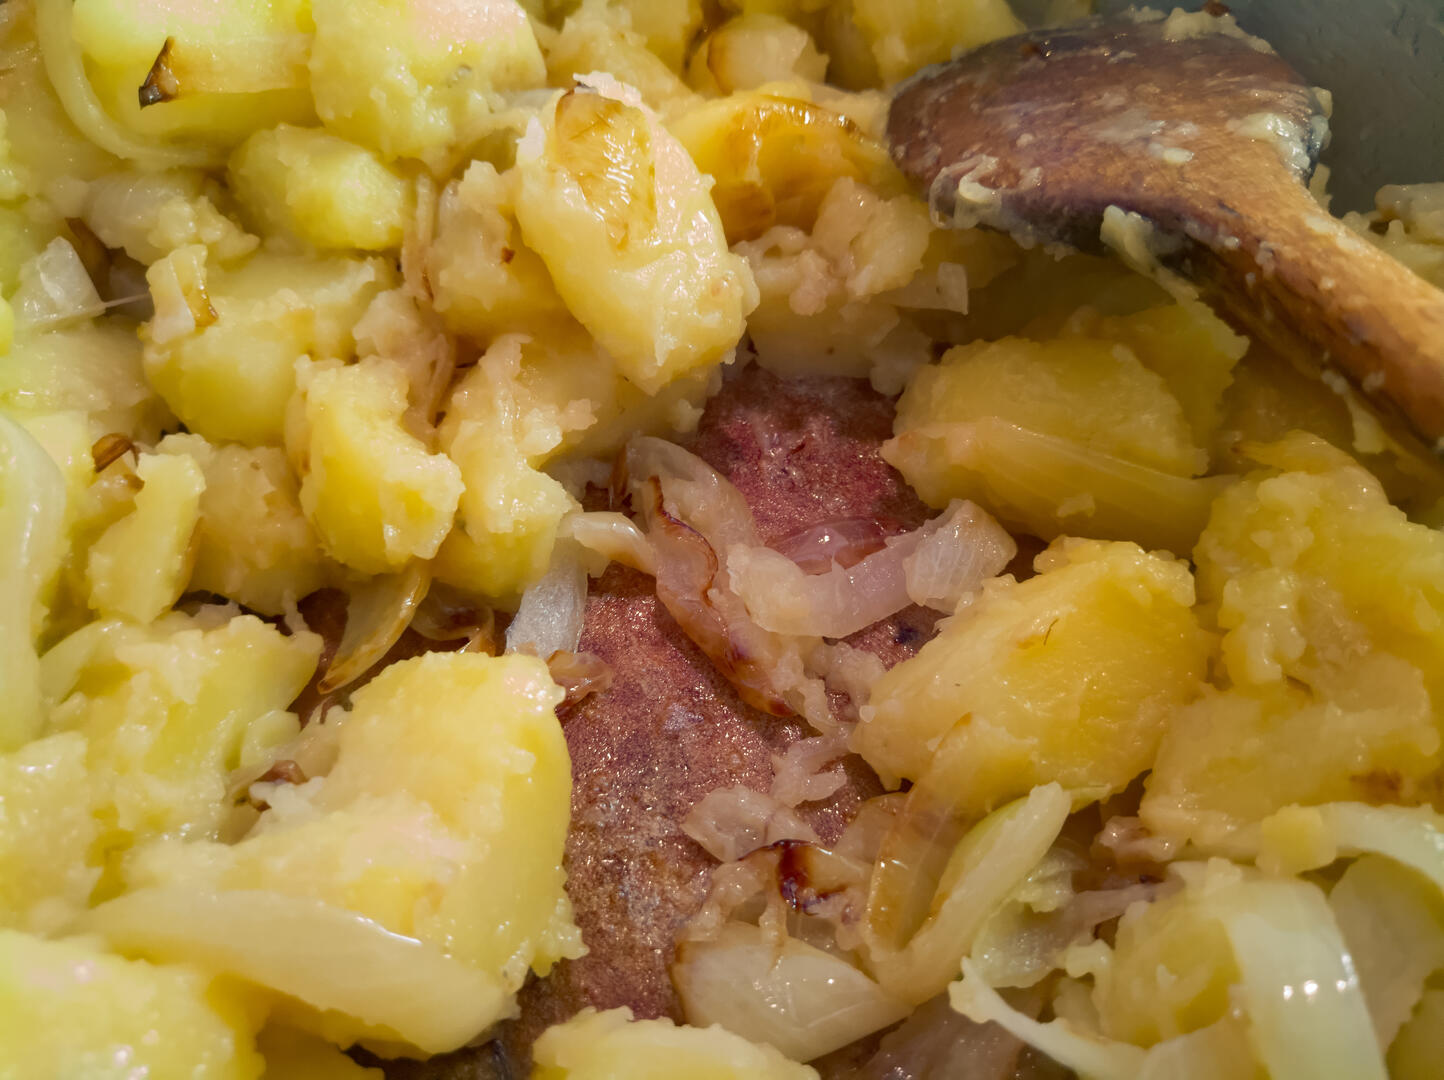
\includegraphics[height=\textheight]{prazen_krompir/IMG_20200409_114616.jpg}}
	    \end{figure}
    
    \introduction{
        This is a side dish that goes well with a nice roast or a \href{https://en.wikipedia.org/wiki/Carniolan_sausage}{Carniolan sausage}. Or eat it on its own, I’m not your mom.
        
        \textbf{\large Potatoes}
        
        Get the butteriest yellow potatoes you can find. Other potatoes may work, buy you’ll get pretty poor results with the starchier varieties.
        
        \textbf{\large Onion}
    
        Yellow or white works fine, red will completely ruin the color.
    }
    
    \ingredients[3]{
        2--3 & Medium potatoes \\
        1 & Medium to large onion \\
        & Salt and pepper
    }
    
    \preparation{
        \step Put whole, unpeeled, potatoes in water and bring to a boil. Boil until soft (test with fork or knife, knork is fine, spork is not; should take about 35 min.)
        
        (You can cook the potatoes well in advance and letting them cool makes them easier to peel.)
        
        \step Peel the potatoes. Cut them into mouthful-sized chunks. Slice the onion into rings or semi-circles.
        
        \step In a pan, fry the onion on high in a bit of oil until it starts to brown. Keep lightly stirring it so it browns, but doesn't burn, until most of it has at least some browning.
        
        \step Add the potatoes and salt, and lower the heat. Here is the tricky part: start stirring and scraping the potatoes off the bottom of your pan. You will not be able to get it ALL off and you should start to build a nice brown crust of potato on the bottom of your pan. THIS IS GOOD\footnote{Just make sure it doesn’t burn. It’s a delicate balance and I would recommend starting on low heat and raising it until it just starts to brown.}.
        
        While you do this, your potatoes will probably start to disintegrate into a chunky mash potato consistency. Keep stirring and building the crust until it’s nice and thick and feels like you will DEFINITELY not be able to scrape that off.
        
        \step Remove from heat, add the pepper\footnote{Pepper, pepper.} and give it one last stir. Cover with a lid and wait.

        \vspace{15em}

        \step The moisture will redistribute and soften your delicious potato crust. You should now be able to peel it off and mix it into the rest of potato-oniony goodness. If it doesn’t come off: cover and wait a bit longer.
        
        \step Serve.
    }
    
\end{recipe}
    \clearpage
    \begin{recipe}
[ %
        preparationtime = {\SI{15}{\minute}},
        bakingtime={\SI{10}{\minute}},
        bakingtemperature={\protect\bakingtemperature{topbottomheat=\SI{175}{\celsius}}},
        portion = {\portion[Cookies]{some}},
        source = {LambMower}
    ]{Cookies}
    
    \ingredients[10]{
        \SI{300}{\gram} & Butter \\
        \SI{2.25}{\deci\liter} & Sugar \\
        \SI{2.5}{\deci\liter} & Brown baking sugar \\
        2 & Eggs \\
        3\,tsp & Vanilla sugar \\
        \SI{7.5}{\deci\liter} & All-purpose Flour \\
        1\,tsp & Salt \\
        1\,tsp & Baking soda \\
        \SI{200}{\gram} & Chocolate of choice that’s been chopped chunky (I used baking milk chocolate)
    }

    \preparation{
        \step Melt the butter. 
        
        \vspace{1em}
        
        \step Whisk together the brown baking sugar, egg and vanilla sugar. 
        
        \step Add the butter once it’s not too warm (don’t want scrambled eggs) and whisk together. 
        
        \step Add salt and baking soda.
        
        \vspace{1em}
        
        \step Add the flour one cup at a time. Once the dough is like a giant fudgeball, add your chocolate to the dough and work that over.

        \step Form dough into balls -- about a tablespoon each -- and put them on a baking sheet covered in parchment paper. Press each ball down lightly.
        
        \step Put into oven at \SI{175}{\celsius} for \SI{10}{\minute}. Cookies are brittle when they come out, so wait a minute before transferring to a cooling rack.
    }
    
\end{recipe}
	\clearpage
	\begin{recipe}
[ %
	preparationtime = {\SI{45}{\minute}},
	bakingtime={\SI{30}{\minute}},
	bakingtemperature={\protect%
		\bakingtemperature{topbottomheat=\SI{180}{\celsius},
							fanoven=\SI{160}{\celsius}}
	},
	portion = {\portion[Brownies]{some}},
	source = {HeNine (from Backen mit Liebe)}
	]{Brownies}
	
	\ingredients[]{
		\SI{100}{\gram} & 70\% dark chocolate \\
		\SI{110}{\gram} & Butter \\
		\SI{125}{\gram} & Sugar \\
		\SI{100}{\gram} & Brown sugar \\
		1\,pinch & salt \\
		1\,tsp & Ground vanilla (or vanilla sugar) \\
		2 & Eggs \\
		1 & Yolk \\
		\SI{120}{\gram} & Flour \\
		3\,tbsp & Cocoa powder
	}
	
	\preparation{
		\step Preheat the oven to \SI{180}{\celsius}. Line $\SI{18}{\centi\meter}\times\SI{18}{\centi\meter}$ (or equivalent) pan with parchement paper.

		\step In a double boiler melt butter and chocolate, mix in both types of sugar, and the salt.
		
		Wait for the mixture to cool a bit so it doesn't cook the eggs.
		
		\step Mix in the vanilla, eggs and the yolk.
		
		\vspace{1em}
		
		\step Sift in the flour and cocoa powder. Stir just enough to combine all the ingredients.
		
		\step Pour the mixture into the pan and smooth it out. Bake for \SI{30}{\minute} or until a toothpick stuck in the middle comes out with moist crumbs.
		
		Unlike cakes, the brownies should still be a bit moist in the center, so take them out before they bake completely through. If the tootpick comes out with a smear of dough, though, give it a bit more time.
		
		\step Let the brownies cool for a bit, then turn them out onto a cooling rack.
		\vspace{1em}
		
		\step After they are completely cooled cut them into cuboids of desired size. It is recommended that you put them in the fridge overnight to let the moisture redistribute a bit.
	}
\end{recipe}
	\clearpage
	\begin{recipe}
[ %
	preparationtime = {\SI{5}{\hour}},
%	bakingtime={\SI{1}{\hour}},
%	bakingtemperature={\protect\bakingtemperature{topbottomheat=\SI{280}{\celsius}}},
	portion = {\portion{4}},
	source = {lunik}
    ]{Chorizo Stew}

	\ingredients[6]{
		1 & Chorizo ring (~\SI{225}{\gram}) \\
		\SI{1}{\kilo\gram} & Potatoes (something waxy that will stew well) \\
		2 & Medium white onions \\
		\SI{50}{\gram} & Butter \\
		2 cloves & Garlic (optional) \\
		& Salt and pepper (to taste)
	}

	\preparation{
	
		\step Melt butter in pot over medium/medium-high heat.
		
		\step Chop chorizo in to ~\SI{1}{\centi\meter} thick rings and add to pot. Add garlic cloves,
		if using.
		
		\step Fry chorizo until it starts to brown. Stir occasionally to ensure
		that chorizo is cooked evenly.
		
		\step Add chopped onions and stir until onion starts to soften.
		
		\vspace{1em}
		
		\step Chop and add potatoes. Add boiling water to pot until ingredients are
		just submerged.
		
		\step Stir and reduce heat to a bare simmer. Cover and leave to cook for
		\SIrange{3}{4}{\hour}, stirring occasionally.
		
		\step Add salt and pepper to taste and serve.
	}
    
\end{recipe}
	\clearpage
	\begin{recipe}
[ %
%	preparationtime = {\SI{}{\hour}},
%	bakingtime={\SI{1}{\hour}},
%	bakingtemperature={\protect\bakingtemperature{topbottomheat=\SI{280}{\celsius}}},
%	portion = {\portion[Item]{1}},
	source = {ekimekim}
    ]{Grand Marnier Strawberries}

	\ingredients[]{
		& Strawberries \\
		& Grand Marnier Cordon Rouge \\
	}

	\preparation{
		\step Take as many strawberries as desired, cut off tops and cut each in half from top to bottom.
		
		\step Place face-up in a shallow bowl.
		
		\vspace{1em}
		
		\step Add Grand Marnier Cordon Rouge to bowl until strawberries covered.
		
		\vspace{1em}
		
		\step Cover with cling wrap and place in fridge for at least a few hours.
		
		\vspace{1em}
		
		\step When ready, pour off the Grand Marnier and enjoy your delicious Grand Marnier infused strawberries.
	}
    
\end{recipe}
	\clearpage
	\begin{recipe}
[ %
%	preparationtime = {\SI{20}{\hour}},
%	bakingtime={\SI{1}{\hour}},
%	bakingtemperature={\protect\bakingtemperature{topbottomheat=\SI{280}{\celsius}}},
	portion = {\portion[Slice]{1}},
	source = {ekimekim}
    ]{Fairy Bread}

	\ingredients[]{
		1\,slice & White bread \\
		& Hundreds and Thousands (google tells me these are also known as "Nonpareils")
	}

	\preparation{
		\step Take sliced white bread. Butter thickly. 
		
		\vspace{1em}
		
		\step Cover in Hundreds and Thousands, then tilt bread vertically to let excess sprinkles fall away. 

		\step Cut diagonally and serve.
	}
    
\end{recipe}
	\clearpage
	\begin{recipe}
[ %
	preparationtime = {\SI{20}{\hour}},
%	bakingtime={\SI{1}{\hour}},
%	bakingtemperature={\protect\bakingtemperature{topbottomheat=\SI{280}{\celsius}}},
	portion = {\portion{4--6}},
	source = {chimingfish (from \href{https://www.bonappetit.com/recipe/mushroom-carbonara}{Bonappetit})}
    ]{Mushroom Carbonara}
    
    \introduction{
		I usually up the mushrooms to \SI{2}{\pound} because I like having a higher shroom:pasta ratio. Also, I can never find orecchiette, so I usually substitute in mediumish sized shells.
	}

	\ingredients[11]{
		\SI{1x1/2}{\pound} & Crimini or button mushrooms \\
		6 clove & Garlic \\
		2 & Medium shallots \\
		\SI{1}{\cup} & Parsley leaves with tender stems (about $\sfrac{1}{2}$ bunch) \\
		5 & Large egg yolks \\
		1 & Large whole egg \\
		\SI{4}{\ounce} & Store-bought pre-grated Parmesan, plus more for serving \\
		\SI{1x1/2}{\teaspoon} & Freshly ground black pepper, plus more for serving \\
		\SI{1/2}{\cup} & Sxtra-virgin olive oil \\
		\SI{1}{\pound} & Orecchiette \\
		& Kosher salt
	}

	\preparation{
		\step Set a large pot of water to boil, salting the water when boiling.
		
		\step Meanwhile, tear off and discard the stems of the mushrooms and tear the mushrooms into halves or quarters. Lightly smash and thinly slice the garlic, finely chop the shallots, and coarsely chop the parsley.
		
		\step Heat another large pot over medium high heat for ~\SI{3}{\minute} (Dutch ovens work well here). Add the olive oil and mushrooms, and toss to coat. Cook, stirring every \SIrange{4}{5}{\minute} or so, until mushrooms are golden brown, ~\SIrange{13}{18}{\minute}. Note that the mushrooms will release a lot of liquid, and you want to cook at least most, if not all of it off.
		
		\step Meanwhile, put the egg yolks, egg, Parmesan, and pepper in a bowl and whisk together until combined. Set aside.
		
		\step Once the mushrooms have been cooking for ~\SI{10}{\minute}, add your pasta to the salted boiling water. Cook until ~\SI{2}{\minute} short of \textit{al dente}.
		
		\step After the mushrooms have finished browning, add the garlic, shallots, and \SI{1x1/2}{\teaspoon} salt to the mushrooms. Cook, stirring often, for ~\SI{1}{\minute}.
		
		\step Once pasta is ~\SI{2}{\minute} off \textit{al dente}, reserve ~\SI{2}{cups} of pasta water, then drain the pasta. 
		
		\step Add the pasta and ~\SI{1}{\cup} of water to the mushrooms, and cook over medium-low heat for ~\SI{2}{\minute}, stirring often. After this, remove from heat and let cool for \SI{1}{\minute}.
		
		\step Add ~\SI{1/2}{\cup} of the pasta water to the egg mixture, and whisk to combine. 
		
		\vspace{1em}
		
		\step Gradually add the egg mixture to the pasta, stirring vigorously, and add some more pasta water if the sauce is still too thick. 
		
		\step Stir in the parsley, salt to taste, and serve with more Parmesan/pepper.
	}
    
\end{recipe}
	\clearpage
	\begin{recipe}
[ %
	preparationtime = {\SI{1x1/2}{\hour}},
%	bakingtime={\SI{1}{\hour}},
%	bakingtemperature={\protect\bakingtemperature{topbottomheat=\SI{280}{\celsius}}},
	portion = {\portion{6--8}},
	source = {chimingfish},
	sourceref = {\href{https://www.bonappetit.com/recipe/digaag-qumbe-yogurt-coconut-chicken}{Bonappetit}}
    ]{Digaag Qumbe}

	\pretitle{{\color{gray}\Large Yogurt-coconut chicken}\vspace{-1.5ex}}

    \introduction{
    	I've never actually tried serving over spinach, I usually just do rice. Also, I usually leave out the ghee, and I use plain Greek yogurt.
	}

	\ingredients[22]{
		3 & Medium tomatoes (about \SI{6}{cups}) \\
		1 & Red bell pepper \\
		2 & Jalape\~nos \\
		\SI{1/2}{\cup} & Extra-virgin olive oil \\
		2 & Onions \\
		2 & Large garlic cloves \\
		1 & \SI{1}{\inch} piece fresh ginger (about \SI{1}{\tablespoon}) \\
		\SI{1}{\tablespoon} & Curry powder \\
		\SI{1}{\tablespoon} & Ground cumin \\
		\SI{1}{\teaspoon} & Ground turmeric \\
		\SI{1/4}{\teaspoon} & Ground cardamom \\
		& Kosher salt \\
		\SI{1}{\cup} & Plain yogurt \\
		\SI{1}{\tablespoon} & Tomato paste \\
		1 & Yukon Gold potato\\
		1 & Carrot \\
		\SI{2}{\pound} & Skinless, boneless chicken thighs \\
		1 & \SI{14}{\ounce} can of coconut milk \\
		\SI{3}{\tablespoon} & Ghee (optional) \\
		\SI{1}{\cup} & Cilantro, plus whole leaves for serving \\
		& Steamed rice and/or spinach (for serving) \\
		& \textbf{Optional:} Bananas for serving \\
	}

	\preparation{
		\step Remove seeds and membranes from the bell pepper and, optionally\footnote{If you want less heat.}, jalape\~nos, and coarsely chop both along with tomatoes.

		\step Blend tomatoes, bell pepper, and jalapeños in a blender or food processor until almost smooth; set aside.

		\step Heat oil in a large pot over medium. Add chopped onion and finely chopped garlic and cook, stirring often, until beginning to soften; about \SI{5}{\minute}.

		\step Add peeled and finely chopped ginger, cumin, curry powder, turmeric, and cardamom; season generously with salt. Cook, stirring, until very fragrant; about \SI{1}{\minute}.

		\step Add reserved tomato mixture to pot and stir well to combine. Stir in yogurt and tomato paste, cover pot, and simmer 10 minutes.

		\step Add potato -- peeled and cut into \SI{3/4}{\inch} cubes -- and carrot -- peeled, cut into \SI{1/4}{\inch}-thick coins -- and continue to cook, stirring occasionally, until vegetables are nearly tender, \SIrange{15}{18}{\minute}.

		\step Add chicken cut into \SI{1}{\inch} pieces, coconut milk, ghee (if using), and \SI{1}{\cup} coarsely chopped cilantro. Stir to combine, then simmer until chicken is tender and sauce thickens, about \SI{20}{\minute}.

		(Make sure to simmer with an uncovered pot here to allow water to evaporate off.)

		\step Season with salt. Divide rice among bowls. Spoon chicken, vegetables, and sauce over. Top with cilantro leaves.

		\textbf{Optional:} Serve with a banana.
	}

\end{recipe}
	\clearpage
	\begin{recipe}
[ %
	preparationtime = {\SI{1}{\hour}},
	bakingtime={\SIrange{20}{24}{\minute}},
	bakingtemperature={\protect\bakingtemperature{topbottomheat=\SI{350}{\fahrenheit} (\SI{175}{\celsius})}},
	portion = {\portion[Muffins]{18--20}},
	source = {chimingfish}
    ]{Apple Muffins}
    
    \introduction{
    	I usually cut down the granulated sugar to \SI{1.5}{cups}. 
    	
    	Any baking apple will do here, although Granny Smith is probably a good standby? 
    	
    	Also, I'd say that a mixer isn't strictly necessary here, although it is nice if you have one.
	}

	\ingredients[13]{
		\SI{2}{cups} & Granulated sugar (1.5 for a less sweet muffin) \\
		2 & Large eggs \\
		\SI{1}{\cup} & Vegetable oil \\
		\SI{1}{\tablespoon} & Vanilla extract \\
		\SI{3}{cups} & All-purpose flour \\
		\SI{1}{\teaspoon} & Salt \\
		\SI{1}{\teaspoon} & Baking soda \\
		\SI{1}{\teaspoon} & Ground cinnamon \\
		\SI{3}{cups} & Peeled, cored, diced apples (around 3 apples) \\
		& Brown sugar for topping (around \num{1/2} cup)
	}

	\preparation{
		\step Preheat oven to \SI{350}{\fahrenheit} (\SI{175}{\celsius}) and line muffin pan with 18--20 paper liners.
		
		\step With a mixer, cream together sugar, eggs, oil, and vanilla. The mixture should be a pale yellow.
		
		\step In a separate bowl, whisk together flour, baking soda, salt, and ground cinnamon. 
		
		\step Add dry ingredients to creamed mixture and mix until combined. The batter will be very thick almost like the texture of cookie dough. Mix in the diced apples. The dough will loosen up a bit when the apples are mixed in.
		
		\step Fill paper liners almost to the top, about \num{3/4} of the way full. Sprinkle each muffin top generously with brown sugar.
		
		\step Bake at \SI{350}{\fahrenheit} (\SI{175}{\celsius}) for \SIrange{20}{24}{\minute}.
	}
    
\end{recipe}
	\clearpage
	\begin{recipe}
[ %
	preparationtime = {\SI{2}{\hour}},
%	bakingtime={\SI{1}{\hour}},
%	bakingtemperature={\protect\bakingtemperature{topbottomheat=\SI{280}{\celsius}}},
	portion = {\portion[Gyros]{4--5}},
	source = {chimingfish},
	sourceref = {\href{https://www.the-girl-who-ate-everything.com/chicken-gyros-opa/}{The Girl Who Ate Everything}}
    ]{Chicken Gyros}

    \introduction{
    	I usually cook the chicken using my broiler.

    	If you're using a regular to particularly thick chicken breast, I recommend either butterflying it or pounding it thin with the flat side of a meat tenderizer before marinating it so that it'll cook more quickly and evenly later.

    	Finally, the tzatziki can be made further ahead of time and the chicken can be marinated for longer than an hour if desired.
	}

	\ingredients[19]{
		\multicolumn{2}{c}{\textbf{Tzatziki sauce:}} \\
		\SI{1}{\cup} & Plain Greek yogurt \\
		1 & Regular cucumber peeled and seeded \\
		\SI{1}{\teaspoon} & Minced garlic \\
		\SI{1}{\teaspoon} & White wine vinegar \\
		& Salt and pepper \\
		& Squeeze of fresh lemon juice \\
		& Extra virgin olive oil \\
 		\multicolumn{2}{c}{\textbf{For the chicken:}} \\
 		\SI{1x1/4}{\pound} & Boneless skinless chicken breasts \\
		\SI{2}{\teaspoon} & Minced garlic \\
		& Juice of 1 lemon (\SIrange{2}{3}{\tablespoon}) \\
		\SI{2}{\teaspoon} & Red wine vinegar \\
		\SI{2}{\tablespoon} & Extra virgin olive oil \\
		\SI{2}{\tablespoon} & Plain Greek yogurt \\
		\SI{1}{\tablespoon} & Dried oregano \\
		& Salt and pepper \\
		\multicolumn{2}{c}{\textbf{To assemble:}} \\
		& Pita bread \\
		& Fresh tomatoes, seeded and diced \\
		& Red onion, sliced thin \\
		& Feta cheese, crumbled
	}

	\preparation{

		\textbf{Tzatziki sauce}

		\step Shred the cucumber or chop in food processor. Wrap in a towel and squeeze to remove as much water as possible.

		\step Mix together the yogurt, shredded cucumber, garlic, white wine vinegar, salt and pepper to taste, and lemon juice. Drizzle lightly with olive oil.

		\step Refrigerate for at least \SI{30}{\minute} before serving to allow the flavors to meld.

		\textbf{Chicken}

		\step Combine the garlic, lemon juice, red wine vinegar, olive oil, yogurt, oregano, and salt and pepper to taste in a medium bowl. Whisk together until mixed well.

		\step Add the chicken pieces to the bowl and mix well to coat.

		\step Cover and refrigerate for about \SI{1}{\hour}.

		\vspace{1em}
		\pagebreak

		\step Cook the chicken as desired, either in the skillet or with the broiler.

		\vspace{1em}

		\step Once the chicken is completely cooked through, transfer to a plate and let rest for \SI{5}{\minute}.
	}

\end{recipe}
	\clearpage
	\begin{recipe}
[ %
	preparationtime = {\SI{3}{\hour}},
	bakingtime={\SIrange{1x1/2}{2}{\hour}},
	bakingtemperature={\protect\bakingtemperature{topbottomheat=\SI{425}{\fahrenheit} (\SI{220}{\celsius}) lower to \SI{350}{\fahrenheit} (\SI{175}{\celsius})}},
	portion = {\portion[Pie]{1}},
	source = {Roosevelt}
    ]{Pumpkin Pie}

    \introduction{
    	You can make your own crust, but my crusts aren't any better than frozen.
	}

	\ingredients[]{
		\SI{1x1/4}{cups} & Pumpkin Puree (fresh is way better but additional moisture
		adds baking time, canned is OK, but not as good) \\
		\SI{3/4}{\cup} & Sugar \\
		\SI{1/2}{\teaspoon} & Salt \\
		\SI{1/2}{\teaspoon} & Ground ginger \\
		\SI{1}{\teaspoon} & Ground cinnamon \\
		\SI{1}{\teaspoon} & All-purpose flour \\
		2 & Eggs \\
		\SI{1}{\cup} & Evaporated milk, undiluted \\
		\SI{1/2}{\teaspoon} & Vanilla extract \\
		& \SI{9}{\inch} Unbaked frozen pie crust
	}

	\preparation{
		\step In a bowl, combine the pumpkin puree, sugar, salt, ginger, cinnamon, flour and eggs. Mix until eggs are broken up.

		\step Add evaporated milk and vanilla extract, and mix until uniform.

		\step Pour into the pie crust.

		\vspace{1em}

		\step Bake at \SI{425}{\fahrenheit} (\SI{220}{\celsius}) for \SI{15}{\minute} then bake at \SI{350}{\fahrenheit} (\SI{175}{\celsius}) until the crust starts to brown
		and the pie isn't jiggly in the center when shaken (\SIrange{1x1/2}{2}{\hour},
		depending on oven and moisture).

	}

\end{recipe}
	\clearpage
	\begin{recipe}
[ %
	preparationtime = {\SI{30}{\minute}},
%	bakingtime={\SI{1}{\hour}},
%	bakingtemperature={\protect\bakingtemperature{topbottomheat=\SI{280}{\celsius}}},
	portion = {\portion{4--8}},
	source = {Roosevelt}
    ]{Chicken Drumsticks}
    \introduction{
    	Do not use light soy sauce, nor Kikkoman -- actual stuff that's labeled dark soy sauce; we used Kikkoman at PAX and it didn't work as well.

    	You can scale this recipe a bit depending on how much you need.
	}

	\ingredients[]{
		4--8 & Chicken drumsticks \\
		\SI{1/4}{\cup} & Dark soy sauce \\
		\SI{12}{\ounce} & Can Coke
	}

	\preparation{
		\step Simmer meat in a pot for \SIrange{20}{25}{\minute}.
	}

\end{recipe}
\end{document}